\chapter{T cell receptor affinity in acute vs. chronic pathogen control}
\label{sec:AvC}

With the exception of the preface, the work presented in this chapter constitutes our submitted manuscript, under review at the time of writing, titled ``\secbfcolor{Chronic infection control relies on T cells with lower foreign antigen binding strength generated by N-nucleotide diversity}'' by H. Jamaleddine, D. Rogers, G. Perreault, D. Patel, J.N. Mandl, and A. Khadra. Video files referenced throughout the text can be found in the online preprint of our manuscript, available in~\cite{jamaleddine2022chronic}.


\phantomsection
\section*{Preface}
\addcontentsline{toc}{section}{Preface}

Chapter~\ref{sec:Tr1} outlined the work we had done to understand immunoregulation by therapeutically expanded Tr1 cells. We showed that Tr1 efficacy, based on its antigen specificity and avidity within autoimmune tissues/draining lymph nodes, could largely explain pMHC-NP therapy outcomes from a variety of experimental treatment protocols. Upon completion of this study, we became interested in delving deeper into the role that antigen specificity, and in particular pMHC binding strength, plays in shaping immune responses, this time in the context of infectious pathogen control. More specifically, we wanted to adapt our model presented in Chapter~\ref{sec:Tr1} to try to answer a new set of questions: how do pMHC binding strength distributions, defined along a continuum between the bounds set by positive and negative selection, evolve over the course of an infection, and how might this differ depending on infection duration? Furthermore, can TCR repertoire diversification through non-templated nucleotide additions by TdT (as described in Chapter~\ref{sec:intro_overview_TCRdiversification}) alter the distribution of TCR binding strengths to pMHC, and if so, how might this affect T cell-mediated control of an acute vs. a chronic replicating pathogen? In this chapter, I will outline the modelling work we have done, in collaboration with experimental support generated by the Mandl laboratory, to address these very questions.

\newpage
\section{Abstract}

The breadth of pathogens to which T cells can respond is determined by the T cell receptors (TCRs) present in an individual’s repertoire. Although more than 90\% of the sequence diversity among TCRs is generated by terminal deoxynucleotidyl transferase (TdT)-mediated N-nucleotide addition during V(D)J recombination, the benefit of TdT-altered TCRs remains unclear. Here, we computationally and experimentally investigated whether TCRs with higher N-nucleotide diversity via TdT make distinct contributions to acute or chronic pathogen control. When T cells with high pMHC reactivity have a greater propensity to become functionally exhausted than those of low pMHC reactivity, our computational model predicts a shift toward T cells with low pMHC reactivity over time during chronic, but not acute, infections. This TCR-affinity shift is critical, as the elimination of T cells with lower pMHC-reactivity \textit{in silico} substantially increased the time to clear a chronic infection. Corroborating an affinity-centric benefit for TCR diversity, in experiments using TdT-deficient mice we showed that infection with a chronic viral pathogen led to increased viral loads later in infection, while acute viral control was unaffected. Taken together, our model and experimental data suggest that TdT-mediated TCR diversity is of particular benefit in the control of prolonged pathogen replication.


\section{Introduction}

The generation of lymphocyte receptor diversity is a key feature of adaptive immunity~\cite{cooper2006evolution,schatz2011recombination}. For T cells, this diversity is established by somatic recombination of the V(D)J gene segments that constitute the \textalpha- and \textbeta-chains of the T cell receptor (TCR)~\cite{schatz2011recombination}. The T cell response to any one pathogen consists of a number of T cell clonotypes, each expanded from a rare antigen-specific T cell defined by the unique TCR they express. Every T cell clonotype in a given anti-pathogen response recognizes the same or different antigens in the form of peptides presented by major histocompatibility complexes (pMHC)~\cite{yassai2009clonotype} and T cell clonotypes can differ in their ligand binding strengths by several orders of magnitude~\cite{andargachew2018cd4,kolawole2020relationship}. Recent evidence suggests that heterogeneity among responding T cells in their TCR binding affinity to pMHC, henceforth referred to as pMHC reactivity, correlates with important differences in effector function. For instance, pMHC binding strength in CD4\pos{} T cells has been shown to impact early effector lineage differentiation~\cite{snook2018tcr,ditoro2018differential,van2016tcr}, while among CD8\pos{} T cells it correlates with both their ability to induce target cell lysis and proliferative capacity, and also impacts memory T cell development~\cite{kolawole2020relationship}. However, to what extent the pMHC-reactivity distribution of the T cells that constitute a given response affects how quickly a pathogen can be cleared remains incompletely understood.

Experimental techniques are currently limited in their ability to comprehensively study the temporal evolution of T cell clonotype frequencies with distinct pMHC reactivities that make up the antigen-specific response. One common method of identifying antigen-specific T cells is by pMHC-tetramers, which primarily tag clonotypes on the higher end of the pMHC-reactivity spectrum, while missing most low affinity T cells~\cite{andargachew2018cd4}. Employing pMHC-tetramers also requires \textit{a priori} knowledge of the epitope recognized by the T cell population being investigated – tracking only the T cells that are specific to one epitope rather than the entire population of responding T cells. Two-dimensional (2D) binding assays measuring TCR-ligand binding affinity similarly rely on knowing the specific epitope recognized by the T cells under study~\cite{huang2010kinetics}. Tracking T cell responses by focusing on only a subset of epitope-specific T cells can therefore introduce biases and disregards the contribution of the remaining pathogen-specific T cell population. Complementing experimental results with a theoretical framework that accounts for pMHC reactivity in a T cell repertoire is thus a useful approach to obtaining a clearer understanding of the mechanisms impacting pMHC-reactivity profiles and, consequently, T cell responses to infection.

A critical contribution to the diversification of the T cell repertoire in all jawed vertebrates is made by a DNA polymerase, called terminal deoxynucleotidyl transferase (TdT), that adds non-templated nucleotides to the V(D)J junctions in \textalpha\textbeta{TCRs}~\cite{schatz2011recombination,gilfillan1995mice,cabaniols2001most,litman2010origins}, enhancing TCR repertoire diversity $\sim$10 fold from the germline recombinatorial diversity alone~\cite{davis1988t,murugan2012statistical,zarnitsyna2013estimating}. However, the benefit of the N-diversification mediated by TdT has remained elusive given that TdT-knockout (KO) mice have shown no increased susceptibility to infection, nor any detectable impairment in their response to challenge with an acute pathogen~\cite{gilfillan1995efficient,gilfillan1995mice}. Interestingly, the genetic sequence and structure of TdT is highly conserved across vertebrates~\cite{lee1994isolation,hansen1997characterization}, suggesting a hitherto unclear evolutionary benefit for its mechanism of action. One hypothesis proposed is that TdT introduces TCRs that, on average, possess lower reactivity to foreign pMHC~\cite{vrisekoop2014revisiting}. Indeed, TdT KO T cells are more efficiently positively selected in the thymus~\cite{gilfillan1994more}, suggesting they may have inherently greater pMHC affinity. Moreover, upon influenza A virus infection, the HA\textsubscript{518} epitope-specific CD8\pos{} splenic T cells from TdT KO mice were about 10 times more sensitive to antigenic stimulation as measured by IFN\textgamma{} production than epitope-specific CD8\pos{} T cells from wild type mice, again consistent with the idea that TdT-independent TCRs have higher ligand affinity~\cite{haeryfar2008terminal}. Importantly, during chronic antigen stimulation in infection and cancer mouse models alike, T cells with higher pMHC-reactivity have been shown to be more prone to exhaustion, whereby their cytokine production and contribution to pathogen or tumour control is substantially impaired over their low-affinity counterparts~\cite{wherry2003viral,alexander1996role,shakiba2021tcr}. Thus, TdT-dependent TCRs may confer an advantage during chronic infections if the more germline TCRs with higher pMHC-reactivity are more likely to become exhausted and ineffective.

Here, we sought to generate a theoretical framework to examine the role of heterogeneity in T cell reactivity to foreign pMHC in the clearance of an acute or chronic pathogen. To predict the impact of a TdT-deficient T cell repertoire on infection outcomes, we developed and implemented a computational model capturing the kinetics of both acute and chronic pathogen replication that also explicitly considered the evolution of TCR affinity distributions during infection. Our simulations showed that, during chronic infection, there was a decrease in the average pMHC reactivity of the antigen-specific T cell population. Importantly, our model suggested that when the TCR repertoire lacked T cells with lower pMHC reactivity, pathogen clearance during chronic, but not acute, infection was delayed. In line with these model predictions, chronic lymphocytic choriomeningitis virus (LCMV) infection of mice with TdT KO T cells led to more protracted viral replication and a significant delay in viral clearance. Taken together, our modeling and experimental results support the notion that one evolutionary benefit of TdT may be to increase the frequency of T cells with lower pMHC reactivity, and in doing so providing better control of ongoing pathogen replication during chronic infection and preventing them from persisting for longer periods of time within the host.


\section{Results}

\subsection{T cell population model captures kinetics of viral load for both acute and chronic infections}

\begin{figure}[htb!]
    \centering
    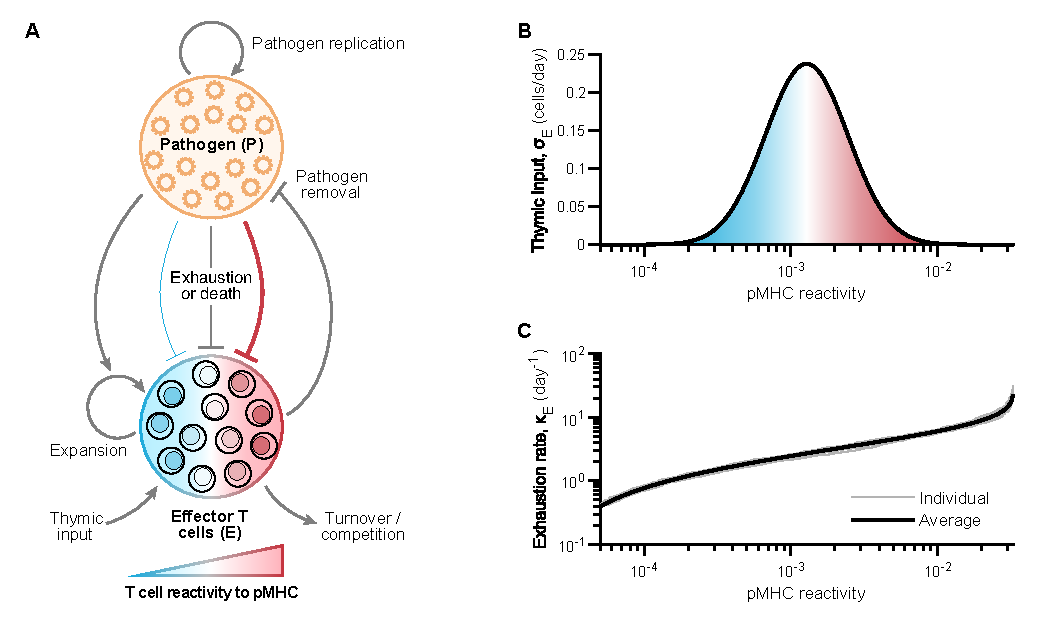
\includegraphics[width=\textwidth]{Figures/AvC/fig1_scheme.pdf}
    \caption[Implementing a computational population model defining the dynamics of pathogen replication and responding T cell clonotypes]{\textit{Implementing a computational population model defining the dynamics of pathogen replication and responding T cell clonotypes}. %
    %
    \secbfcolor{(A)}~Model scheme illustrating model variables and their interactions. The model is described by a system of integro-differential equations that govern the rates of change of the two key players, namely pathogen loads ($P$) and the effector T cells ($E$) that are specific for pathogen-derived antigens in the form of pMHC. The effector T cell population, encompassing the complete collection of pathogen-specific CD4\pos{} and CD8\pos{} T cells, are defined on a continuum according to their overall reactivity to pMHC ($a_k$), i.e., the strength of the overall TCR-pMHC interactions (the shade from blue to red represents the reactivity continuum of T cells to pMHC that ranges from low to high TCR affinities, respectively). Pathogen load is subject to replication as well as negative regulation by effector T cells. Effector T cells expand upon pathogenic exposure, with a constant low-level thymic input, natural turnover, and inter-cellular competition. Pathogen persistence promotes T cell exhaustion and/or activation-induced cell death, with higher pMHC-reactivity T cells more susceptible to these than their low pMHC-reactivity counterparts. For simplicity, we (i)~left out the role of other players such as antigen-presenting cells and B cells from the model in order to focus on the specific role of pMHC reactivity in defining dynamics, and~(ii) did not explicitly distinguish between the action of CD4\pos{} and CD8\pos{} T cells. %
    %
    \secbfcolor{(B,~C)}~Functions depicting pMHC reactivity-dependent parameter values, wherein thymic input~(B), $\sigma_E=f(a_k)$, mimics the shape of a theoretical log-normal distribution, and T cell exhaustion rate~(C), $\kappa_E$, is determined by sampling from a shifted exponential distribution of a set mean, and sorted in ascending order by assigning smaller depletion rates to T cells of low pMHC-reactivity, and vice versa, producing variability between model simulation runs (shown by gray traces obtained from 25 individual model simulations).}
    \label{fig:AvC_scheme}
\end{figure}

In order to compare the temporal evolution of pMHC reactivities of responding T cell clonotypes during acute and chronic infections, we first needed a simple computational model that could recapitulate the kinetics of both rapidly cleared and prolonged pathogen replication. We developed a model that could replicate the serum viral loads obtained upon infection with two strains of LCMV that differ by only 3 coding point mutations, Armstrong (LCMV-Arm) and Clone 13 (LCMV-Cl13), and produce the time course of acute and chronic viral loads in the host, respectively~\cite{wherry2003viral,bergthaler2010viral,ahmed1984selection}. Importantly, the single amino acid mutations between LCMV-Arm and -Cl13 do not occur in peptide segments from which known T cell specific pMHC epitopes are derived~\cite{abdel2019viruses,kotturi2007cd8+} and thus different infection outcomes are governed exclusively by viral replication dynamics within infected cells~\cite{abdel2019viruses,bergthaler2010viral}. Our model considered key interactions between the pathogen load ($P$) and the pMHC-reactivity continuum of all responding effector CD4\pos{} and CD8\pos{} T cells ($E$) (Fig.~\ref{fig:AvC_scheme}A). The dynamics of $P$ and $E$ depend on the rates of pathogen replication, T cell proliferation and expansion upon antigen encounter, thymic input, homeostatic T cell turnover, and pathogen-induced exhaustion and/or cell death (Fig.~\ref{fig:AvC_scheme}A). To incorporate pMHC reactivity explicitly into our model, we defined the thymic input into the effector T cell pool, $\sigma_E$, to be a function of pMHC reactivity (denoted $a_k$, Fig.~\ref{fig:AvC_scheme}B), a parameter proportional to the strength of TCR signaling (refer to Methods) whereby $a_k$ represents how likely it is that a T cell will proliferate upon antigenic stimulation~\cite{standifer2009changes}. Consistent with previous studies, we assumed that the strength of negative regulatory mechanisms (such as T cell exhaustion and activation-induced cell death) is positively correlated with the pMHC reactivity of a given T cell~\cite{wherry2003viral,alexander1996role,shakiba2021tcr}. Variability in model outcomes is generated by randomization of this T cell exhaustion rate, which is selected from a shifted exponential distribution and sorted in increasing order as a function of pMHC reactivity (with a mean determined by model fitting, see Methods) (Fig.~\ref{fig:AvC_scheme}C).

Model parameters (Table~\ref{tab:AvC_parameters}) were obtained by fitting simulated pathogen loads to serum data of LCMV infections from Wherry et al.~\cite{wherry2003viral} using a genetic algorithm (Fig.~\ref{fig:AvC_supp_timeSeries}A,~B). Given that previous work showed LCMV-Cl13 replicates more rapidly in infected cells than LCMV-Arm~\cite{bergthaler2010viral}, we set the replication rate (denoted $r_P$) for our simulated chronic viral infection to be higher than for the acute infection, while keeping all other parameters consistent between the two conditions. By modulating only the pathogen replication rate, we produced time courses that qualitatively matched both LCMV-Arm and LCMV-Cl13 replication dynamics (Fig.~\ref{fig:AvC_timeSeries}A,~B, and Fig.~\ref{fig:AvC_supp_timeSeries}A,~B).
%
\begin{figure}[htb!]
    \centering
    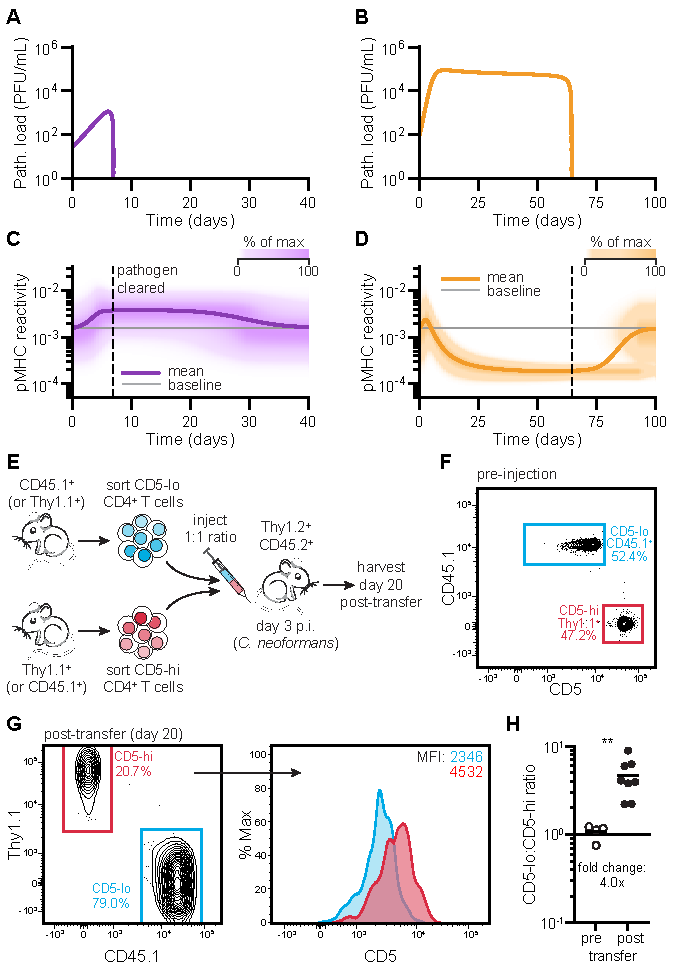
\includegraphics[width=0.64\textwidth]{Figures/AvC/fig2_timeSeries.pdf}
    \caption[T cell pMHC reactivity evolution over time during a T cell response differs between acute and chronic infections]{%
    \textit{T cell pMHC reactivity evolution over time during a T cell response differs between acute and chronic infections}. %
    %
    \secbfcolor{(A-D)} Simulations of pathogen loads and T cell levels in time during acute~(A,~C) or chronic~(B,~D) infection, showing time series simulations of pathogen loads~(A,~B) and heat maps representing the relative proportion of T cells across pMHC reactivities~(C,~D). Overlaid traces represent the mean pMHC-reactivity value in time, with the baseline value denoted in gray. Dotted black lines denote the time at which the pathogen is cleared. %
    %
    \secbfcolor{(E)}~Schematic of experimental approach illustrating adoptive cell transfer of a 1:1 ratio of CD5\supr{lo} and CD5\supr{hi} na\"{i}ve CD4\pos{} T~cells (either Thy1.1\pos{} or CD45.1\pos{}) into congenic CD45.2\pos{} Thy1.2\pos{} recipient mice infected 3 days prior with chronic \textit{C. neoformans}. %
    %
    \secbfcolor{(F,~G)}~Representative flow cytometry plot of CD5\supr{lo} CD45.1\pos{} and CD5\supr{hi} Thy1.1\pos{} transferred T cell populations, pre-injection into recipient infected mice~(F), or 20 days post-transfer with CD5 expression levels shown as a histogram and mean fluorescent intensities (MFI) indicated in blue and red text~(G). %
    %
    \secbfcolor{(H)}~Ratio of transferred CD5\supr{lo} to CD5\supr{hi} T~cells, pre-injection or 20 days post-transfer. **, P = 0.004 computed using a two-tailed Wilcoxon rank sum test, data from 2 independent experiments (n=8 mice).}
    \label{fig:AvC_timeSeries}
\end{figure}
%
In our simulations, the acute viral load peaked at 6.0~days post infection, followed by rapid clearance around 6.9~days post infection based on 100 trial simulations (Fig.~\ref{fig:AvC_timeSeries}A, and Fig.~\ref{fig:AvC_supp_timeSeries}C). In contrast, increasing the viral replication rate to simulate chronic viral replication resulted in prolonged infections with a median time to clearance of 64 days (based on 100 trial simulations) (Fig.~\ref{fig:AvC_timeSeries}B, and Fig.~\ref{fig:AvC_supp_timeSeries}C). Thus, our model was able to reproduce pathogen loads characteristic of both acute and chronic infections by modifying only the rate of pathogen replication while keeping all other model parameters constant.

\subsection{Chronic infection skews responding T cell clonotypes toward lower pMHC reactivities}

Having developed our \textit{in silico} model of acute and chronic pathogen infection, we next asked how the pMHC-reactivity profile of the antigen-specific T cell population evolved over time in each case. When we simulated effector T cell responses to acute infection, we found that the pMHC-reactivity profile of T cells shifted toward a higher pMHC-reactivity mean until peak pathogen replication was reached, followed by a gradual return to baseline after the infection was resolved (Fig.~\ref{fig:AvC_timeSeries}C, and Mov.~\ref{mov:AvC_timeSeries}). Of note, the return of the pMHC-reactivity mean value to the pre-infection baseline was a result of omitting a memory T cell compartment from the model, since our focus was on the effector phase of the T cell response. The shift we observed in the pMHC-reactivity profile during acute infection agrees with previous experimental studies showing that T cells with greater pMHC reactivity expand to large numbers more readily upon antigenic stimulation~\cite{busch1999t,king2012t,rosenthal2012low,mandl2013t}.

Next, we investigated whether the dynamics of pMHC reactivity among responding T cell clonotypes differed during chronic infection. In contrast to acute infection, the pMHC-reactivity distribution peaked during the early phases of chronic infection but was followed by a substantial shift toward lower pMHC reactivities, before returning to baseline after infection clearance (Fig.~\ref{fig:AvC_timeSeries}D). This indicated that, as more T cells of high pMHC reactivity became functionally exhausted due to chronic antigen stimulation from persistent virus (and were thus removed from the active effector T cell pool), T cells of progressively lower reactivities to pMHC gradually predominated among responding T cell clonotypes (Fig.~\ref{fig:AvC_timeSeries}D, and Mov.~\ref{mov:AvC_timeSeries}).

To further investigate whether our model was consistent with experimental data, at least for CD4\pos{} T cells, we used a previously identified surface marker proxy for pMHC reactivity, CD5, whose expression level on CD4\pos{} T cells correlates with pMHC binding strength as measured by tetramer fluorescent intensity and whose expression level is maintained post activation~\cite{mandl2013t,azzam1998cd5,rogers2021pre}. We sorted na\"{i}ve CD4\pos{} T cells on the 20\% CD5\supr{lo} and CD5\supr{hi} cells, as previously described~\cite{mandl2013t,rogers2021pre}, mixed the two sorted populations at a 1:1~ratio (identified by congenic markers, CD45.1 or Thy1.1), and adoptively transferred the mix to CD45.2\pos{} Thy1.2\pos{} recipient mice that were infected 3 days earlier with \textit{Cryptococcus neoformans}, a persistent pulmonary fungal pathogen~\cite{schneider2020migration} (Figs.~\ref{fig:AvC_timeSeries}E,~F, and Fig.~\ref{fig:AvC_supp_timeSeries}D,~E). In contrast to what was previously described during acute infections, where the CD5\supr{hi} CD4\pos{} T cells predominated the response on day 8 post infection~\cite{mandl2013t}, in the later stage of the anti-\textit{Cryptococcus} CD4\pos{} T cell response in the lung, the CD5\supr{lo} CD4\pos{} T cells outnumbered CD5\supr{hi} CD4\pos{} T cells 4-fold (Fig.~\ref{fig:AvC_timeSeries}G,~H).

In summary, our modeling results suggest that the temporal evolution of pMHC reactivities of T cells contributing to the response to an acute compared to a chronic infection is distinct, with T cells of lower pMHC reactivities predominating during the chronic infection phase, whereas T cells of greater pMHC reactivity predominate during an acute infection. Our experimental data from CD4\pos{} T cells corroborated this result and is consistent with evidence from studies of both antigen-specific CD4\pos{} and CD8\pos{} T cells that T cells with lower pMHC reactivity predominate during chronic infection~\cite{gallegos2016control,schober2020reverse,tsitsiklis2020unusual}. 

\subsection{The distribution of pMHC reactivities of responding T cells impacts time to infection clearance}

Having established that the pMHC reactivity of effector T cells changed differentially in acute versus chronic infection, we wanted to determine whether the reverse is true, i.e., whether altering the pMHC-reactivity profile of the antigen-specific T cell population would lead to changes in the duration of pathogen replication upon infection using our simulations. To accomplish this, we targeted model parameters affecting either the mode or the span of the T cell pMHC-reactivity distribution to investigate how perturbing these two parameters impact the T cell response to a pathogen. In these simulations, we maintained the pathogen replication rate at a constant value obtained from fitting the model to LCMV-Cl13 viral loads, and used the time at which pathogen burden returned to zero post infection as a measure to assess: (i)~class of infection (i.e., acute vs. chronic), and (ii)~effectiveness of the T cell response in clearing infection. Gradually varying the mode of the pMHC-reactivity profile over 40~logarithmically spaced values between~$10^{-4}$ and~$10^{-2}$ and running 50~independent simulations per mode value revealed three distinct clusters with different durations of infection (Fig.~\ref{fig:AvC_dists}A).
%
\begin{figure}[t]
    \centering
    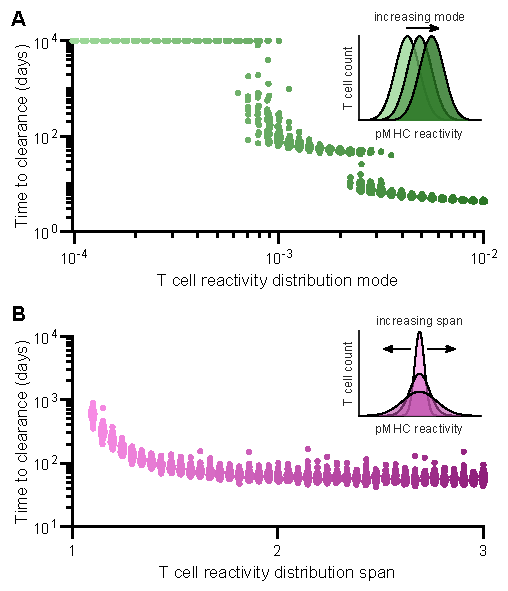
\includegraphics[width=0.48\textwidth]{Figures/AvC/fig3_distributionEffs.pdf}
    \caption[Mode and span of the naïve T cell pMHC-reactivity profile impact pathogen clearance times]{\textit{Mode and span of the naïve T cell pMHC-reactivity profile impact pathogen clearance times}. %
    %
    \secbfcolor{(A, B)}~Time required to clear a replicating pathogen in silico when varying the mode~(A), and the span~(B) of the initial T cell count as a function of pMHC reactivity. Each data point shows the result of a single simulation trial for a given, randomized set of parameters for T cell exhaustion ($\kappa_E$) as determined by the relation defined in Fig.~\ref{fig:AvC_scheme}C. Insets schematically indicate how the T cell count of the starting (pathogen-free/baseline) configuration, as a function of pMHC reactivity, is altered by increasing its mode~(A) or span~(B). The distribution mode and span shown are equivalent to $e^{-(\mu+\sigma^2 )}$ and $e^\sigma$, respectively, where $\mu$ and $\sigma$ are, respectively, the mean and standard deviation of the log-normal pMHC reactivity function defining thymic input (for full details, see Section~\ref{sec:AvC_modelParsFitting}).}
    \label{fig:AvC_dists}
\end{figure}
%
Variability between different runs of the model arise from the randomization of the exhaustion rate, $\kappa_E$, in each simulation, as described previously (Fig.~\ref{fig:AvC_scheme}C). When the mode of antigen-specific pMHC-reactivities of the T cell repertoire was too low (less than $7\E{-4}$), the infection persisted indefinitely, indicating that T cells failed to clear the pathogen. At intermediate values of pMHC reactivity (between $7\E{-4}$ and $2\E{-3}$) the time to clearance was around 100~days, comparable to chronic LCMV-Cl13 infection. When reactivity to foreign pMHC was high, the infection was cleared within 10~days, representative of an acute infection (Fig.~\ref{fig:AvC_dists}A). Varying the span of the pMHC reactivity distribution also affected pathogen replication kinetics, with narrow pMHC reactivity distributions exhibiting impaired chronic pathogen clearance compared to T cell repertoires with broader distributions (Fig.~\ref{fig:AvC_dists}B).

Taken together, our results demonstrate that the pMHC-reactivity profile of responding T cells during infection has a pronounced effect on determining infection duration, with outcomes ranging from rapid pathogen clearance to the complete failure of the T cell response to resolve the infection. Of note, rather than observing gradual shifts in the time to clearance with \textit{in silico} manipulations of the pMHC-reactivity profile, we found sharp jumps between different infection clearance times (namely from acute to chronic, and chronic to indefinitely persistent). By reducing the model to a one-clone, 2-dimensional system of ordinary differential equations and performing bifurcation analysis (Fig.~\ref{fig:AvC_supp_bfns}), we found that distinct solution trajectories through state space are responsible for producing separate clusters of infection durations. Importantly, analysis of the one-clone model showed that, exclusively in the case of chronic pathogen load, the evolution of the T cell profile toward lower pMHC reactivities is responsible for the eventual resolution of chronic infection (Fig.~\ref{fig:AvC_supp_bfns} and Mov.~\ref{mov:AvC_nullclines}, see Section~\ref{sec:AvC_2DmodelAnalysis}).

\subsection{Absence of T cells with low pMHC-reactivity generated by N-nucleotide diversity delays the clearance of chronic infection.}

Our results thus far showed that an increased contribution from T cell clonotypes with low pMHC reactivity could be important in clearing chronic, but not acute, infections. Thus, we next investigated whether populating a TCR repertoire exclusively with higher pMHC reactivity T cells would affect the clearance of either an acute or a chronic infection \textit{in silico}. We tackled this question in two ways. First, in our simulations, we removed T cells with lower pMHC reactivity by eliminating all T cells possessing a pMHC reactivity value below a predefined cut-off threshold without altering the total number of responding T cells, and then progressively increased this threshold to remove up to half of the pMHC reactivity distribution (Fig.~\ref{fig:AvC_modelKO}A). %
%
\begin{figure}[tb]
    \centering
    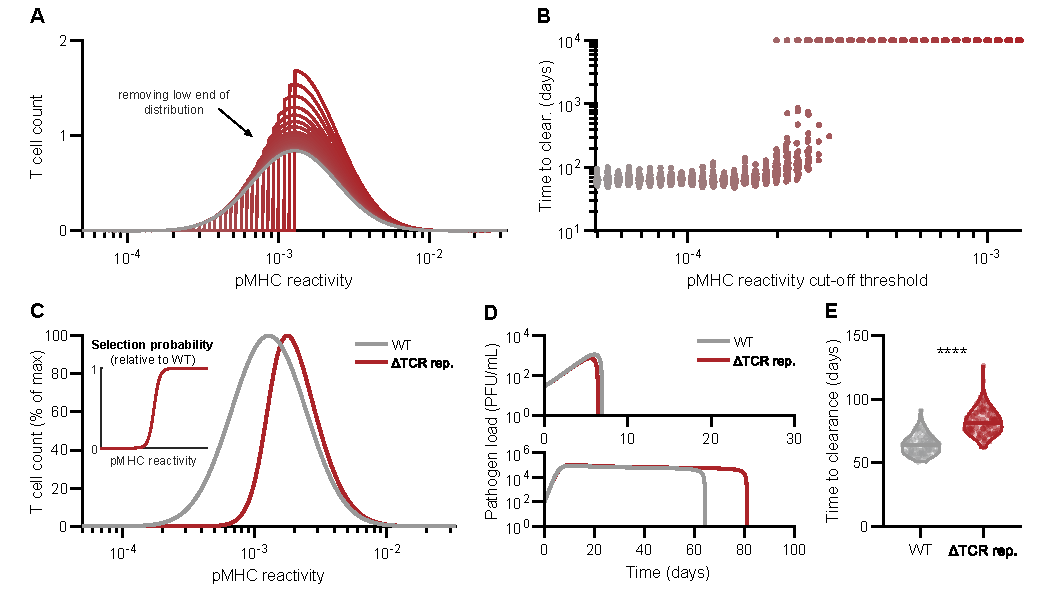
\includegraphics[width=\textwidth]{Figures/AvC/fig4_modelKO.pdf}
    \caption[Deficiency in TCRs with low pMHC-reactivity in silico leads to prolonged chronic, but not acute, pathogen replication]{%
    \textit{Deficiency in TCRs with low pMHC-reactivity in silico leads to prolonged chronic, but not acute, pathogen replication}. % 
    %
    \secbfcolor{(A)}~Distributions of T cells as a function of pMHC reactivity obtained by successively removing low-affinity T cells using different cut-off thresholds from the model’s starting configuration, while keeping the total number of T cells conserved, until only the upper half of the distribution remained. These starting configurations were generated by setting all values of the thymus input, $\sigma_E$, for T cells below a given pMHC-reactivity threshold to 0. \textbf{(B)}~Time to pathogen clearance as a result of increasing the cut-off threshold for T cell reactivity to pMHC corresponding to the configurations shown in A. For each cut-off threshold, 50 simulation trials were performed as described in Fig.~\ref{fig:AvC_dists}. %
    %
    \secbfcolor{(C)}~Theoretical T cell pMHC-reactivity configuration of an altered TCR repertoire (denoted \dTCR{} repertoire) deficient in low-affinity T cells relative to the WT configuration. The \dTCR{} repertoire was assumed to have a lower thymic selection probability (relative to WT repertoire), implying a lower value of the thymic input parameter, $\sigma_E$, for T cells with low pMHC reactivity (see Methods). Inset: Probability of selection, relative to the WT repertoire, for T cells of the \dTCR{} repertoire, with fewer T cells of low reactivity to pMHC being sourced by thymic selection. %
    %
    \secbfcolor{(D)}~Model simulations comparing representative pathogen load traces of WT (gray) or \dTCR{} repertoire (red) systems during acute (top) or chronic (bottom) infection. %
    %
    \secbfcolor{(E)}~Time to clearance of chronic infections for 100 model simulations from WT and \dTCR{} repertoire systems. ****, P = 1.52\E{-25} computed using the Wilcoxon rank sum test.}
    \label{fig:AvC_modelKO}
\end{figure}
%
Our simulations demonstrated that impeding the shift toward lower TCR affinities during a chronic infection by progressively removing T cells with lower pMHC reactivity in this manner dramatically prolonged the time to clearance for the chronic infection cluster, with higher cut-off thresholds leading to failure to clear the chronic pathogen altogether (Fig.~\ref{fig:AvC_modelKO}B). Interestingly, repeating this analysis while decreasing the pathogen replication rate from 1.22~day$^{-1}$ to 1.17 day$^{-1}$ revealed that high cut-off thresholds could result in rapid pathogen clearance owing to the greater number of only high pMHC reactivity T cells; this, as a result, leads to the formation of an acute infection cluster (Fig.~\ref{fig:AvC_supp_modelKO}A-B). This result is consistent with that of Fig.~\ref{fig:AvC_dists}A, where higher pMHC-reactivity modes can prevent infection chronicity altogether. When the number of high pMHC reactivity T cells was kept unchanged, the acute cluster did not form at high values of the cut-off threshold (Fig.~\ref{fig:AvC_supp_modelKO}C-D).

While gradually removing all effector T cells below a certain pMHC-reactivity threshold allowed us to investigate the distinct roles of T cells with low versus high pMHC reactivity, we next designed a second approach in which we also modified our model to simulate a more biologically plausible change in the pMHC reactivity profile. In this approach, we defined an altered TCR repertoire (\dTCR{} rep.), wherein the probability that low-reactivity T cells selected for in the thymus was reduced, while the selection probability of high-reactivity T cells was left relatively unchanged (Fig.~\ref{fig:AvC_modelKO}C). We found that this \dTCR{} rep. did not alter replication kinetics of an acute pathogen (Fig.~\ref{fig:AvC_modelKO}D, top). However, testing the \dTCR{} rep. model with a chronic pathogen revealed that chronic infection clearance was impaired (Fig.~\ref{fig:AvC_modelKO}D, bottom), and time to clearance was significantly longer (Fig.~\ref{fig:AvC_modelKO}E). In summary, altering the pMHC-reactivity profiles of responding T cells by introducing reductions in T cells with low pMHC-reactivity showed that modulating only the TCR repertoire pMHC reactivity led to impaired control of chronic, but not acute, infections.

The proposed hypothesis that N-diversity mediated by TdT, which accounts for 90-95\% of the TCR repertoire diversity~\cite{cabaniols2001most}, disproportionately generates lower-affinity TCRs~\cite{vrisekoop2014revisiting} has been difficult to address experimentally without a specific prediction of the type of infection that these low-affinity TCRs are important for with regard to curtailing pathogen replication. Based on our modeling results suggesting that a TCR repertoire deficient in T cells with low pMHC reactivity would lead to an impaired effector T cell response during chronic infection, we next sought to test our model prediction \textit{in vivo} in mice and ask whether TdT might benefit the host by promoting the shift of T cells from high- to lower-pMHC reactivity. Given that TdT also inserts non-templated nucleotides into the B cell receptor during B cell development~\cite{jackson2013shape}, and the altered B cell receptor repertoire might therefore impact viral clearance, we restricted the TdT-deficiency to the T cell compartment only, with B cells expressing normal levels of TdT. To do so, we generated bone marrow chimeras (Fig.~\ref{fig:AvC_tdtKO}A) whereby TCR\textbeta{} KO bone marrow was mixed 1:1 with either WT bone marrow (leading to development of WT B and T~cells), or with bone marrow obtained from TdT and JH double KO mice (leading to the development of WT B~cells and TdT KO T~cells).%
%
\begin{figure}[t]
    \centering
    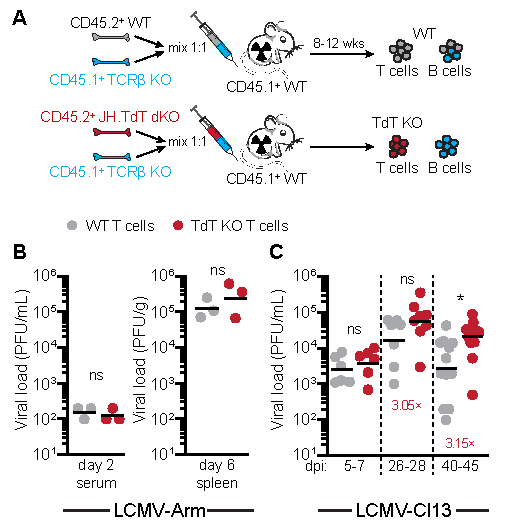
\includegraphics{Figures/AvC/fig5_tdtKO.pdf}
    \caption[Loss of TdT restricted to T cells in vivo impairs control of chronic, but not acute, infections]{\textit{Loss of TdT restricted to T cells in vivo impairs control of chronic, but not acute, infections}. %
    %
    \secbfcolor{(A)}~Generation of bone marrow chimeric mice possessing WT B~cells, and either WT T~cells (reconstitution of irradiated mice with 1:1 ratio of bone marrow from WT mice and TCR\textbeta{}\KO{} mice) or TdT KO T~cells (reconstitution with 1:1 ratio of bone marrow from JH and TdT double KO mice and TCR\textbeta{}\KO{} mice). %
    %
    \secbfcolor{(B)}~LCMV-Arm viral loads in the serum (left) and spleen (right) of mice with WT or TdT KO T cells measured at 2 or 6 days post-infection, respectively (n=3 mice per group). %
    %
    \secbfcolor{(C)}~LCMV-Cl13 viral loads in the serum of mice with WT or TdT KO T cells in early (5-7 days post-infection), mid (26-28 days post-infection) or late (40-45 days post-infection) stages of viral replication (n=6-18 mice per group). Fold-changes of viral loads in mice with TdT-deficient T cells, relative to WT, are indicated. *, P = 0.013 computed using a Kruskal-Wallis test.}
    \label{fig:AvC_tdtKO}
\end{figure}
%
We verified that our bone marrow reconstitutions led to a 1:1 ratio of hematopoietic cell development from each of the donors, identified using congenic markers (Fig.~\ref{fig:AvC_supp_tdtKO}A). In line with previous results from full TdT KO mice in response to acute LCMV infection~\cite{gilfillan1995efficient}, we observed no differences in the viral load following LCMV-Arm infection between the WT T cell and TdT KO T cell groups, both 2~days post infection in the serum, and 6 days post infection in the total spleen homogenate (Fig.~\ref{fig:AvC_tdtKO}B). In contrast, mice with TdT KO T~cells had a significantly higher viral load (3.15-fold increase) during the chronic phase (day 40-45) following infection with LCMV-Cl13 (Fig.~\ref{fig:AvC_tdtKO}C). Since irradiated bone marrow recipients still retain some endogenous hematopoietic stem cells, we repeated the above experiment using TCR\textbeta{} KO recipient mice instead (i.e., mice lacking endogenous \textalpha{}\textbeta{}T cells), and obtained similar results where chimeras with TdT KO T cells had a 3.74-fold increase in viral load by day~41 post-infection (Fig.~\ref{fig:AvC_supp_tdtKO}B-C).

Previous experimental and theoretical studies alike have shown that limiting the breadth of the T cell response to infection, or introducing “gaps” in the TCR repertoire, can impede pathogen control~\cite{meyer2004limited,van2011costimulatory,van2013rate}. We therefore wanted to investigate whether introducing similar gaps in the context of our pMHC-reactivity model could equally recapitulate the viral load data in mice with TdT KO T cells, demonstrating impaired chronic (but not acute) pathogen control. To test this, we constructed an alternative \dTCR{} repertoire where we decreased the number of T cell clonotypes 10-fold, without affecting the overall affinity profile or the total population size of the precursor pool (Fig.~\ref{fig:AvC_supp_alternativeKO}A). Interestingly, when we simulated both acute and chronic infections using this alternative \dTCR{} repertoire configuration, we found no differences in pathogen clearance in either case (Fig.~\ref{fig:AvC_supp_alternativeKO}B-C), inconsistent with what we saw in mice with TdT KO T~cells (Fig.~\ref{fig:AvC_tdtKO}). Incidentally, we also tested whether decreasing T cell precursor frequencies 10-fold instead (evenly across all pMHC-reactivity values) might recapitulate our experimental results, but again found a mismatch between the data and the simulations wherein acute, and not chronic, infection control seemed to be impaired relative to the WT configuration (Fig.~\ref{fig:AvC_supp_alternativeKO}D-F). Thus, while our modelling does not rule out the possibility for additional, affinity-independent advantages of TCR repertoire diversification by TdT, when taken together these results lend further support to notion that TdT benefits hosts challenged with chronic infections, and that it does so, at least in part, by generating T cells with lower affinity for foreign pMHC.



\section{Discussion}
\label{sec:AvC_discussion}

N-nucleotides added by TdT during V(D)J gene segment recombination contribute enormously to the diversification of the TCR repertoire~\cite{cabaniols2001most}. Yet, despite the fact that TdT is found in all jawed vertebrates with adaptive immune systems studied thus far~\cite{litman2010origins}, the specific contexts in which these non-germline TCRs are better poised to control pathogen replication have not been clear~\cite{gilfillan1995mice,gilfillan1995efficient}. Here we combined computational modelling and experimental approaches to investigate the temporal evolution of pMHC reactivities of responding T cells during infection and its impact on pathogen clearance. We developed a computational model that 1.~produced time courses characteristic of infections with both acute and chronic pathogens, and 2.~incorporated a continuum-affinity formalism to track T cell pMHC-reactivity distributions over time.  Using the \textit{in silico} model we developed, we made two predictions that we tested experimentally. First, we showed that, while in acute infection T cells with high pMHC reactivity predominate~\cite{busch1999t,bachmann1997functional,mcheyzer1995antigen}, during chronic infection T cells with low pMHC reactivity contribute disproportionately. Second, we found that the removal of low pMHC-reactivity T cells leads to a delay in chronic, but not acute, pathogen clearance in the model, which we replicated in infected mice when T cells were TdT-deficient. Importantly, our data corroborate prior experimental work showing no differences in clearance by TdT KO mice of the acute viral pathogens Vesicular Stomatitis, Sendai, Influenza A, and LCMV-WE~\cite{gilfillan1995efficient,haeryfar2008terminal}. Thus, while it has been proposed that a TdT-deficient TCR repertoire may have specific ‘holes’ with regard to antigen specificities represented, this has so far not been supported by experimental evidence. Indeed, without accounting for possible differences in T cell clonotype precursor frequencies, our model predicts longer times to clearance for chronic pathogens. Our work therefore suggests a hitherto undescribed benefit for TCR repertoire diversification by TdT in chronic infection control.

A TdT-deficient repertoire and its consequences for pathogen control are relevant not only for understanding the broad evolutionary conservation of TdT across vertebrates, but also in the context of neonatal immunity, given that the TCR repertoire is initially generated in the absence of TdT. TdT expression is first detected in thymocytes in mice and humans 3-5~days after birth and after 20 weeks of gestation, respectively~\cite{bonati1994tcr,bogue1992regulation}. Lacking N-nucleotide additions, neonatal TCR sequences are shorter, are more likely to be shared between individuals (public)~\cite{yassai2000thymocyte,yassai2002molecular} and are more cross-reactive~\cite{gavin1995increased}. Interestingly, in line with TdT KO T cells having greater pMHC reactivity, it has been shown that the neonatal repertoire is more self-reactive due to a greater affinity for pMHC, and neonatal T cells more prone to tolerance~\cite{rudd2020neonatal}. To what extent the neonatal TCR repertoire versus other epigenetic or transcriptional differences described in neonatal compared to adult T cells play a role in altered responses to infection requires further analysis.

Although we fit our model to viral replication data from acute and chronic strains of LCMV~\cite{wherry2003viral}, its conclusions may be generalizable to other pathogens. For instance, we found that following infection with the pulmonary fungal pathogen, C. neoformans, CD4\pos{} T cells with low self-pMHC reactivity, and thus low foreign reactivity~\cite{mandl2013t}, predominated among the responding effector T cells during the chronic infection phase. These experimental findings expand on previous work suggesting that, during chronic infection, T cells with lower pMHC-reactivity predominate in both CD4\pos{}~\cite{gallegos2016control} and CD8\pos{}~\cite{schober2020reverse,tsitsiklis2020unusual} T~cells. Notably, in our current model we did not distinguish between CD4\pos{} and CD8\pos{} T~cell responses, and it is possible that there are key differences between these T~cell subsets with regard to the role of TdT and functional biases among TdT-generated TCRs, which need to be further explored. Moreover, our model did not consider memory T cells following pathogen clearance, and experimental data suggests that memory T cells are differentially selected for in terms of their reactivity to pMHC, resulting in a final steady-state pMHC-reactivity distribution of memory T cells that differs from the starting na\"{i}ve T cell pMHC reactivity distribution~\cite{andargachew2018cd4,busch1999t,mandl2013t}. Of note, while our model does not include all aspects of the host-pathogen response, such as the effects of host age-related changes in T cell precursor sizes and responses, phenotypic complexities of different stages of T cell exhaustion, antigen abundance and immunodominance hierarchies, and pathogen evolution to evade host immunity~\cite{rouse2010immunity,mclane2019cd8,yewdell2006confronting}, the model could be extended by incorporating some of these additional phenomena in order to study their individual contributions to the control of acute or chronic pathogens in the context of a pMHC-reactivity continuum. Additionally, the effect of TdT deficiency in the B~cell receptor repertoire and its impact on acute or chronic pathogen clearance would be interesting to investigate in future studies.

Our work revealed the effects of varying features of the pMHC-reactivity distribution of responding T cells on pathogen clearance and suggested a differential role between T cells with low- and high-reactivity to pMHC during different phases of the immune response. This is particularly intriguing, given recent observations that in both mice and humans, both CD4\pos{} and CD8\pos{} T cells with lower self-pMHC reactivity (low CD5 surface levels) express higher levels of \textit{Dntt}, the gene encoding TdT~\cite{rogers2021pre,sood2021cd5,fulton2015tcr}. Thus, differences in TdT expression level during development in individual thymocytes may ultimately contribute to the numbers of N-nucleotides inserted into the recombining TCR and be a critical variable impacting strength of pMHC reactivity. To provide additional insight into whether there are indeed different roles for TdT-mediated versus germline-encoded TCRs during infection, comprehensive TCR sequencing studies will be a powerful tool. Indeed, recent work using machine learning has shown that CD4\pos{} T cells with higher self-pMHC-reactivity have fewer N-nucleotide additions on average when compared to T cells with lower reactivity to pMHC, and that longer TCR sequences with a greater number of N-nucleotide additions predominate in chronic infection~\cite{textor2022machine}. Overall, our model formalism provides a foundation for further studies of T cell pMHC-reactivity distributions over the course of an immune response, and it will be particularly interesting to investigate whether, as our model suggests, TdT-dependent TCRs are important in the control of other chronic pathogens and are perhaps making underappreciated contributions in settings such as cancer and autoimmunity.


\section{Materials and Methods}

\subsection{Mice}

C57BL/6, congenic CD45.1\pos{}, congenic Thy1.1\pos{}, and TCR\textbeta{}\KO{} mice~\cite{mombaerts1992mutations} were purchased from Jackson Laboratories (Bar Harbor, ME). The TdT\KO{} mice were shared by Dr. A. Feeney (The Scripps Research Institute)~\cite{gilfillan1993mice} and the JH\KO{} mice were shared by Dr. J. Fritz (McGill)~\cite{gu1993independent}. All mice were on a C57BL/6 background, bred in-house and experiments performed at 6-12 weeks of age with both males and females. Animal housing, care, and research were in accordance with the Guide for the Care and Use of Laboratory Animals and all procedures performed were approved by the McGill University Animal Care Committee.

\subsection{Pathogen stocks and infections}

\subsubsection{LCMV}

LCMV-Arm and -Cl13 strains were propagated from stocks provided by Dr. M. Richer (University of Indiana) on BHK-21 or L929 cells (ATCC). Briefly, virus was added at MOI 0.01, incubated for 90 minutes in serum-free media at 37\degree{C} in 5\% CO\sub{2}, then topped up with complete media for incubation for another 48 hours before harvesting the supernatant. BHK-21 cells were cultured in EMEM supplemented with 0.1\% penicillin/streptomycin, 1\% L-glutamine, 1\% non-essential amino acids, 1\% sodium pyruvate, and 10\% FBS and maintained at 37\degree{C} in 5\% CO\sub{2}. L929 cells were cultured in RPMI supplemented with 10\% FBS, 1\% L-glutamine, and 1\% penicillin/streptomycin. Mice were infected with 2\E{5} plaque forming units (PFU) of LCMV-Arm by intra-peritoneal injection or 2\E{6} PFU by intravenous injection for LCMV-Cl13 as previously described~\cite{wherry2003viral,richer2013pathogen}. Mice were bled by either tail artery or cardiac puncture into sterile Eppendorf tubes kept on ice, blood was spun down at 12,000 rpm for 10 minutes and serum aliquoted and frozen for viral titer determination. Spleens were collected in 1\% RPMI and weighed. Spleens were placed in Lysing Matrix D tubes (MP Biomedicals) and homogenized with a MagNA Lyser (Roche) at 6000 rpm for 40 seconds. Spleen homogenate was then spun down at 12,000 rpm for 10 minutes at 4\degree{C} and supernatant was transferred to a separate sterile tube and re-spun at 12,000 rpm for 10 minutes at 4\degree{C} then aliquoted and frozen for viral titer determination. Viral titers (stocks used, mouse serum, and tissue samples) were determined by plaque assay with Vero cells~\cite{ahmed1984selection}. Briefly, Vero cell monolayers were infected with 100 \textmu{}L of serially diluted serum (1 in 10 dilutions from $10^{-1}$ to $10^{-7}$) and incubated for 90~minutes at 37\degree{C} in 5\% CO\sub{2}. Infected cells were then overlaid with 1\% agarose (Wisent) and incubated for 3 days at 37\degree{C} in 5\% CO\sub{2}. A second agarose overlay supplemented with 1\% neutral red was then added and cells incubated for 24~hours at 37\degree{C} in 5\% CO\sub{2}, after which plaques were counted.

\subsubsection{\textit{C. neoformans}}

The H99 strain was provided by K. Kwon-Chung (NIH). Frozen stocks ($-80$\degree{C}) were prepared in 15\% glycerol from fresh cultures from a YPD agar plate. Three days before infection, \textit{C. neoformans} was scraped from the frozen stock and streaked onto a YPD agar plate. One day prior to infection, a single colony was inoculated and incubated for 12-16 hours at 30\degree{C} with continuous agitation in YPD broth. Immediately before infection, \textit{C. neoformans} was resuspended in cold PBS. Mice were then anesthetized with isoflurane and infected by intrapharyngeal aspiration with 5\E{3} colony forming units (CFU) in 20 \textmu{}L of PBS. Mice were sacrificed and tissue collected 23 days after infection. \textit{C. neoformans} CFUs were determined as previously described~\cite{schneider2020migration}.

\subsection{Lymphocyte isolation}

For the C. neoformans infections, prior to harvest an intravascular stain using 2.5 µg anti-CD45 (30F11) was performed as previously described (62). Infected lungs were harvested in cold PBS and minced with scissors. Lung was then digested at 37\degree{C} with agitation for 30 minutes in digestion buffer (1~mg/mL collagenase D, 50~U/mL DNase I, 1~mg/mL hyaluronidase, 1\% L-glutamine, 1\% pen/strep in RPMI). Tissue was then passed through a 100-μm filter with PBS supplemented with 1\% FBS and resuspended in 10~mL of 37\% Percoll in RPMI. Samples were centrifuged at 3000~rpm for 20~minutes at 22\degree{C}. ACK lysis buffer (Life Technologies) was added for 3~minutes, samples washed with PBS, refiltered, and resuspended in complete RPMI (10\% FBS, 1\% L-glutamine, 1\% HEPES buffer, 1\% pen/strep, 1\% sodium pyruvate, 1\% non-essential amino acids, 0.1\% 2-mercapto-ethanol 1000X solution). Dilution of single-cell suspensions at 1:10 in Trypan Blue and manual counting of live cells (Trypan Blue-negative) on a hemacytometer was used to determine total cell counts.

Spleen and peripheral lymph nodes (inguinal, axillary, brachial, and mesenteric) were collected and passed through a 70-μm filter with 1\% RPMI (1\% penicillin/streptomycin, 1\% L-glutamine, and 1\% FBS). ACK lysis buffer (Life Technologies) was added for 3 minutes, samples washed with PBS, refiltered and resuspended in 1\% RPMI. Dilution of single-cell suspensions at 1:10 in Trypan Blue and manual counting of live cells (Trypan Blue-negative) on a hemacytometer was used to determine total cell counts.

\subsection{Bone marrow chimeras}

Bone marrow was collected from the femurs and tibias of donor mice (either JH\KO{} TdT\KO{}, TCR\textbeta{}\KO{}, or B6 WT) by flushing the marrow from the bones with cold 1\% RPMI. Bone marrow cells were then passed through a 70~\textmu{}m filter with 1\% RPMI and red blood cells lysed with ACK lysis buffer (Life Technologies) and cell counts determined as above. Recipient mice (either B6 CD45.1\pos{} or TCR\textbeta{}\KO{} CD45.1\pos{}) were irradiated twice at 550 rads 3 hours apart and reconstituted with a 1:1 mix of 2.5\E{6} cells per genotype that were injected intravenously within 5 hours of the first irradiation. To establish the WT chimera (WT T cells and B cells) B6 and TCR\textbeta{}\KO{} bone marrow cells were mixed at equal proportions; to make the T cell restricted TdT\KO{} chimeras (WT B cells) bone marrow cells from JH\KO{} TdT\KO{} mice were mixed 1:1 with TCR\textbeta{}\KO{} bone marrow cells. Recipient mice were given neomycin water (2~g/L) 2 days prior to bone marrow transfer and kept on the antibiotic water for 2~weeks following transfer. Mice were used 8-12~weeks post irradiation and bone marrow reconstitution.

\subsection{Flow cytometry}

Samples were incubated in Fixable Viability Dye (AF780, Life Technologies) diluted in PBS for 20 minutes at 4\degree{C}. Extracellular antibodies were diluted in FACS buffer (2\% FBS and 5~mM EDTA in PBS) with Fc Block (Life Technologies) and incubated for 30 minutes at 4\degree{C}. For intracellular staining, samples were then incubated in FoxP3 Transcription Factor Fixation/Permeabilization Concentrate and Diluent (Life Technologies) for 30~minutes at 4\degree{C}. Intracellular antibodies were diluted in Permeabilization Wash Buffer (Life Technologies) and samples were incubated for 30-60 minutes at 4\degree{C}. Directly conjugated antibodies used were as follows: TCRb (H57-597), CD4 (RM4.5), CD8a (53-6.7), CD5 (53-7.3), Foxp3 (FJK-16 s), CD44 (IM7), CD62L (MEL-14), CD25 (PC61.5), CD45.1 (A20), CD45.2 (104), PD-1 (29F.1A12), B220 (RA3-6B2), NK1.1 (PK126). For all flow cytometry experiments, cells were acquired using an LSRFortessa (BD Bioscience) and analyzed with FlowJo software (BD Bioscience).

\subsection{Cell sorts}

Cell sorts were performed as previously described~\cite{rogers2021pre}. Briefly, lymphocytes from Thy1.1\pos{} or CD45.1\pos{} congenic mice were isolated in single cell suspension as described. Spleens and lymph nodes (inguinal, axially, brachial, mesenteric, and cervical) were pooled from 15 mice for each congenic marker. Cells were then magnetically enriched for total CD4+ T cells (Stemcell EasySep CD4\pos{} T cell Enrichment kit or Miltenyi Biotec CD4\pos{} T cell Isolation Kit). Enriched CD4\pos{} T cells were stained with surface antibodies for 1~hour at 4\degree{C}. Naive CD4\pos{} T cells were sorted on singlets, CD4\pos{}, CD8\neg{}, CD62L\supr{hi}, CD44\supr{lo}, and 20\% CD5\supr{hi} or CD5\supr{lo}. Sorts were performed on a FACS Aria III (BD Bioscience). All cell populations were sorted to $>$90\% purity.

\subsection{Adoptive cell transfers}

\textit{C. neoformans} infection. All donors and recipients were sex matched. 15 CD45.1\pos{} or Thy1.1\pos{} mice were used as donors to obtain a total of 8-14\E{6} cells for each of 20\% CD5\supr{hi} and 20\% CD5\supr{lo} cells sorted as described above. Sorted CD5\supr{lo} and CD5\supr{hi} were then mixed in a 1:1 ratio. 4-7\E{6} of each sorted population was adoptively transferred into CD45.2\pos{} Thy1.2\pos{} recipients that were infected with 5\E{3}~CFU of \textit{C. neoformans} 3 days prior to transfer. Cells were isolated from the lungs of recipient mice 20 days post-transfer.

\subsection{Statistical analyses of experimental data}

Group comparisons were performed using Prism V9 (GraphPad). The cut-off for significance considered was p$<$0.05. Information about implemented statistical tests and sample sizes for individual experiments is provided in the figure legends.

\subsection{Computational modelling}

To study a continuum of antigen-specific T cell affinities in the context of acute vs. chronic pathogen infections, we used the following system of integro-differential equations based on Fig.~\ref{fig:AvC_scheme}:
%
\begin{align}
    \dv{P}{t} &= r_P P \left( 1 - \frac{P}{P_{\textrm{max}}}\right) - \kappa_P \int_{\kmin{}}^{\kmax{}} E(t,k) \frac{P}{P+a \, k} \, \dd k \label{eq:AvC_P} \\[0.3em]
    \begin{split}
        \pdv{E(t,k)}{t} &= \sigma_E(k) + r_E E(t,k) \frac{P}{P+k} - \delta_E E(t,k) \\
        &\quad- \kappa_E E(t,k) \frac{P}{P+b\,k} - \varepsilon E(t,k) \int_{\kmin{}}^{\kmax{}} E(t,k) \dd k
    \end{split} \label{eq:AvC_E}
\end{align}
%
This was implemented in a manner similar to the models presented in~\cite{jamaleddine2020quantifying,jaberi2015continuum}. In Eqs.~\eqref{eq:AvC_P} and~\eqref{eq:AvC_E}, $P(t)$ represents the pathogen load in time, and $E(t,k)$ represents the time-dependent reactivity-continuum of effector T cells, with T cell pMHC reactivity taken to be proportional to the quantity $1/k$, where $k$ is the pathogen load for half-maximum activation of T cells. To facilitate understanding of pMHC-reactivity distributions, we defined a new, unitless quantity $a_k$ (whose magnitude is equivalent to $1/k$) as a measure for T cell reactivity to pMHC~\cite{standifer2009changes}. While this quantity is related to the overall binding avidity between T cells and APCs, we considered only affinity-related changes in TCR binding strength, and thus used the term pMHC reactivity to avoid confusion with other factors that can affect binding avidity. For simplicity, in Eq.~\eqref{eq:AvC_P} we assumed a logistic growth of the pathogen (with replication rate $r_P$ and carrying capacity $P_\textrm{max}$) as was done in previous models of LCMV infection~\cite{bocharov1998modelling,kecsmir2003clonal}. Clearance of the pathogen by T cells was described by a product of the T cell number ($E$) and an increasing first-order Hill function of pathogen load with a maximum rate $\kappa_P$, and a half-maximum pathogen load $a \cdot k$ (where $a$ is a scaling factor). We impose the condition that the pathogen replication rate ($r_P$) for chronic pathogens to be larger than that for acute pathogens, as suggested previously in the case of LCMV-Cl13 vs. LCMV-Arm, respectively~\cite{bergthaler2010viral,sullivan2011point}.

The terms included in effector cell dynamics of Eq. 2 were pMHC reactivity-dependent thymic input ($\sigma_E(k)$), T cell replication that depends on pathogen load according to a first-order Hill function (with maximum replication rate $r_E$ and half-maximum activation $k$), natural turnover (with a rate $\delta_E$), and an inter-cellular competition term (with a rate $\varepsilon$). The parameter $\kappa_E$ denotes the rate at which the pathogen causes reduction in the number of active effector T cells able to provide anti-microbial immunity, either via T cell exhaustion, activation-induced cell death, or regulatory T cell intervention. The term $b \cdot k$ represents the pathogen load at half the maximum inactivation rate of effector T cells, where $b>1$ is a proportionality constant.

To study the effects of T cell reactivity to pMHC in the context of acute vs. chronic infection, we denoted the spectrum of effector T cells in time by $E(t,k)$, where $k=1/a_k$ is assumed to be proportional to the reciprocal of T cell reactivity to pMHC consistent with~\cite{standifer2009changes}, $\kmax{}$ is the maximum value of $k$ (corresponding to T cells with the lowest reactivity to pMHC) and $\kmin{}$ is the minimum value of $k$ (corresponding to T cells with highest reactivity to pMHC). Equations~\eqref{eq:AvC_P} and~\eqref{eq:AvC_E} are simulated by discretizing the allowable values of pMHC reactivity within the range defined by $1/\kmax{}$ and $1/\kmin{}$, wherein the solution is obtained by integrating a high-dimensional system of ordinary differential equations (see Section~\ref{sec:AvC_numericalSimmulation}).

\subsection{Model parameters and numerical implementation}
The two pMHC reactivity dependent parameters, $\sigma_E$ and $\kappa_E$, were defined to be functions of T cell reactivity to pMHC ($a_k$) (Fig.~\ref{fig:AvC_scheme}B,~C). A bell-shaped function of pMHC reactivity that mimics a log-normal distribution was used to assign values for thymic input $\sigma_E$, while T cell exhaustion $\kappa_E$ was first sampled from an exponential distribution and then sorted in an ascending order (such that higher-affinity T cells are more susceptible to losing their effector functions than their lower-affinity counterparts). This latter claim is supported by the fact that activation-induced cell death~\cite{alexander1996role} and T cell exhaustion~\cite{wherry2003viral,shakiba2021tcr} scale with the strength of antigenic stimulation. The use of a uniform distribution for $\kappa_E$ produced very similar results (Fig.~\ref{fig:AvC_supp_uniformExhaustion}). Table~\ref{tab:AvC_parameters} summarizes the meanings of the different parameters and their values used to generate model results. Model parameters were obtained by genetic algorithm fitting to LCMV-Arm and LCMV-Cl13 serum data adapted from~\cite{wherry2003viral} (Fig.~\ref{fig:AvC_supp_timeSeries}A-B). To simulate the \dTCR{} repertoire shown in Fig.~\ref{fig:AvC_modelKO}C, the thymus input parameter $\sigma_E$ was modulated by an arctan function such that
%
\begin{equation*}
    \sigma_E^{\textrm{\dTCR{}}}(k) = \frac{1}{2} \sigma_E(k) \left[ 1 - \arctan\left( \frac{\log_{10}k - \log_{10}\kmode{}}{0.15} \right) \right],
\end{equation*}
%
where $\kmode{}$ is the value of the parameter $k$ at which $\sigma_E(k)$ peaks, determined by parameter fitting (for more details, see Section~\ref{sec:AvC_modelParsFitting} - Model parameters and fitting). The new parameter $\sigma_E^{\textrm{\dTCR{}}}(k)$ is subsequently renormalized such that the total thymic input across all T cells remains constant, i.e.,
%
\begin{equation*}
    \sigma_E^{\textrm{\dTCR{}}}(k) \rightarrow \sigma_E^{\textrm{\dTCR{}}}(k) \left( \int_{\kmin{}}^{\kmax{}} \sigma_E (k) \, \dd k \right) \Big/ \left( \int_{\kmin{}}^{\kmax{}} \sigma_E^{\textrm{\dTCR{}}}(k) \, \dd k \right).
\end{equation*}

MATLAB was used to simulate the model equations and perform numerical analyses. Steady state and bifurcation analyses were carried out using XPP/AUTO, a freeware available at \url{http://www.math.pitt.edu/~bard/xpp/xpp.html}). Genetic algorithm fitting was performed using Compute Canada’s Cedar cluster. MATLAB codes used to produce violin plots are available at \url{http://github.com/bastibe/Violinplot-Matlab}. All other MATLAB codes used to perform simulations, parameter fitting, and model analyses can be obtained online at \url{http://www.medicine.mcgill.ca/physio/khadralab/Codes/code_PNAS1.html}.


\section{Acknowledgments}

This work was done in Tiohtiá:ke/Montreal on the traditional territory of the Kanien’kehà:ka, a place which has long served as a site of meeting and exchange amongst many First Nations including the Kanien’kehà:ka of the Haudenosaunee Confederacy, Huron/Wendat, Abenaki, and Anishinaabeg. We honour, recognize, and respect these nations as the traditional stewards of these lands and waters. We would like to thank the animal facility staff at McGill University for their excellent care of our animal colony, C. Stegen and J. Leconte at the Cell Vision Core Facility for cell sorting, F. Buytenhuijs and J. Textor at Radboud University for key intellectual input and for conducting separate analyses not included in the paper, and P. Artusa for initial experiments at an earlier stage of the project that were also not included. H.J. was supported by a Post-Graduate Doctoral Award (NSERC) and a B2X Doctoral Award (FRQNT). D.R. was supported by a Frederick Banting and Charles Best Canada Graduate Doctoral Award (CIHR) and a Tomlinson Doctoral Fellowship (McGill). J.N.M. is a Canada Research Chair for Immune Cell Dynamics. This work was supported by NSERC (Discovery Grants \#2019-04520 to A.K. and \#2016-03808 to J.N.M.).

\newpage
\section{Supporting information}

\renewcommand{\thetable}{S\thechapter.\arabic{table}}
\setcounter{table}{0}

\subsection{Supplementary tables and figures}

Table~\ref{tab:AvC_parameters}, supporting figures, legends for supporting movies, and supporting text are included below. Video files for the supporting movies may be downloaded from the manuscript preprint in~\cite{jamaleddine2022chronic}.

\vspace{0.5in}

\begin{table}[ht]
\footnotesize
\centering
\begin{tabular}{p{0.06\textwidth} p{0.53\textwidth} p{0.12\textwidth} p{0.17\textwidth}}
    \hline
    \textbf{Param.} & \textbf{Description}                                             & \textbf{Value(s)} & \textbf{Units} \\
    \hline
    %
    $r_P$ & Maximum pathogen replication rate & 0.77 (acute) & day$^{-1}$ \\
    & & 1.22 (chronic) & \\
    %
    $P_0$ & Initial pathogen load & 28.4 (acute) & PFU~mL$^{-1}$ \\
    & & 98.3 (chronic) & \\
    %
    $P_{\textrm{max}}$ & Pathogen carrying capacity & 1.17\E{5} & PFU~mL$^{-1}$ \\
    %
    $\kappa_P$ & Maximum pathogen removal rate per T cell & 4.94\E{-2} & PFU~(mL~cell~day)$^{-1}$ \\
    %
    $k$ & Pathogen load at half-maximum activation of T cells & Range & PFU~mL$^{-1}$ \\
    %
    $a_k$ & pMHC reactivity parameter (magnitude equal to $1/k$) & Range & unitless \\
    %
    $a$ & Scaling factor of half-maximum constant in pathogen clearance & 1.77\E{-3} & unitless \\
    %
    $\sigma_{E,\textrm{tot}}$ & Total thymic input across all pMHC-reactivity values & 29.7 & cells~day$^{-1}$\\
    %
    $k_{\textrm{mode}}$ & Mode of the pMHC-reactivity function at which thymic input is maximal &  7.8\E{2} & PFU~mL$^{-1}$ \\
    %
    $k_{\textrm{span}}$ & Span of the pMHC-reactivity function & 1.91 & unitless \\
    %
    $r_E$ & Proliferation rate of effector T cells & 3.19 & day$^{-1}$ \\
    %
    $\delta_E$ & Natural turnover rate of effector T cells & 0.28 & day$^{-1}$ \\
    %
    $\kappa_E$ & Pathogen-dependent T cell exhaustion rate - sampled from a shifted exponential distribution $g(k;\mu) + \kappa_{E,\textrm{min}}$ and sorted (highest $a_k$ corresponds to highest $\kappa_E$ value) & $\mu$ = 3.34 & day$^{-1}$ \\
    %
    $\kappa_{E,\textrm{min}}$ & Minimum exhaustion rate & 0.39 & day$^{-1}$ \\
    %
    $b$ & Scaling factor of half-maximum constant of T cell exhaustion & 38.1 & unitless \\
    %
    $\varepsilon$ & Inter-cellular competition rate & 3.24\E{-6} & cell$^{-1}$~day$^{-1}$ \\
    %
    $N$ & Number of T cell clones obtained from discretizing Eqs.~\eqref{eq:AvC_P}-\eqref{eq:AvC_E} (see Section~\ref{sec:AvC_numericalSimmulation} -- Numerical simulation) & 500 & unitless \\
    \hline
\end{tabular}
\caption[Parameter values used in model simulations]{\textit{Parameter values used in model simulations}. Values were determined by fitting model simulations to serum data in acute vs. chronic LCMV infection~\cite{wherry2003viral} using a genetic algorithm.}
\label{tab:AvC_parameters}
\end{table}

\renewcommand{\thefigure}{S\thechapter.\arabic{figure}}
\setcounter{figure}{0}

% Movies
\vspace{0.5in}
\begin{figure}[h]
    \centering
    \captionsetup{name={Movie}}
    \caption[]{\secbfcolor{(A-F)}~Time series simulations of the model during acute (A-C) or chronic (D-F) infection, showing pathogen loads (A,~D), heat maps representing the relative proportion of T cells across pMHC reactivities (B,~E), and evolution of T cell proportions as a function of pMHC reactivity at each time point (C,~F). Overlaid traces in B and E represent the mean reactivity value in time, weighted by the proportion of T cells of given reactivity values. Dotted black lines denote the time at which the pathogen is cleared.}
    \label{mov:AvC_timeSeries}
\end{figure}

\begin{figure}
    \centering
    \captionsetup{name={Movie}}
    \caption[]{\secbfcolor{(A-B)}~Nullclines of the reduced, 2-dimensional, one-clone model plotted in logarithmic (A) and linear (B) scales over time during chronic pathogen replication. Nullclines vary over time since the parameters for pMHC reactivity ($a_k$) and exhaustion rate ($\kappa_E$) of the one-clone model were set to their respective weighted average values across all T cells of the full model at each time point. Given that the relative proportions of T cells of different pMHC reactivity values vary through time in the full model, the weighted averages of these parameters also change over time. Black lines represent pathogen load ($P$) nullclines while the gray line represents the effector T cell ($E$) nullcline. Superimposed in green is the pathogen load and the total T cell count (across all values of pMHC reactivity) simulated from the full model across time. Refer to Section~\ref{sec:AvC_2DmodelAnalysis} - Analysis of the reduced one-clone, 2D model for more details.}
    \label{mov:AvC_nullclines}
\end{figure}

\renewcommand{\thefigure}{S\thechapter.\arabic{figure}}
\setcounter{figure}{0}

\begin{figure}[htbp]
    \centering
    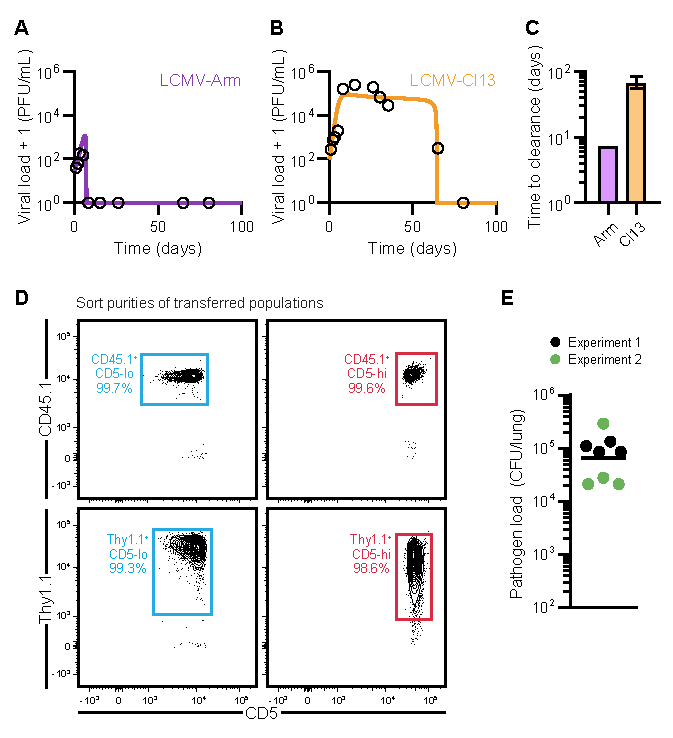
\includegraphics[width=0.64\textwidth]{Figures/AvC/figS1_timeSeries.pdf}
    \caption[Model fitting and adoptive cell transfer experiment set-up details]{\textit{Model fitting and adoptive cell transfer experiment set-up details}. %
    %
    \secbfcolor{(A,~B)}~Serum viral load data in mice infected with LCMV-Arm (A) or LCMV-Cl13 (B) digitized from~\cite{wherry2003viral}, shown as open circles, overlaid on the time series simulations of Eqs.~\eqref{eq:AvC_P}-\eqref{eq:AvC_E}. These simulations were generated using parameter values (Table~\ref{tab:AvC_parameters}) obtained from fitting the model to digitized data shown in (A) and (B) with the implementation of the genetic algorithm (see Section~\ref{sec:AvC_modelParsFitting} - Model parameters and fitting for details). Note that the difference between the two curves was generated by altering the pathogen replication rate parameter and initial pathogen load. %
    %
    \secbfcolor{(C)}~Median time to clearance of 100 simulations for acute and chronic infections (error bars = 95\% confidence intervals). %
    %
    \secbfcolor{(D)}~Flow cytometry panels showing sort purities of transferred CD45.1\pos{} or Thy1.1\pos{} CD5\supr{lo} and CD5\supr{hi} na\"{i}ve CD44\supr{lo} CD62L\pos{} CD4\pos{} T~cells into \textit{C. neoformans} infected mice. %
    %
    \secbfcolor{(E)}~\textit{C.~neoformans} pathogen loads in the lungs of infected mice from 2 independent experiments (n=8 mice).}
    \label{fig:AvC_supp_timeSeries}
\end{figure}

\begin{figure}
    \centering
    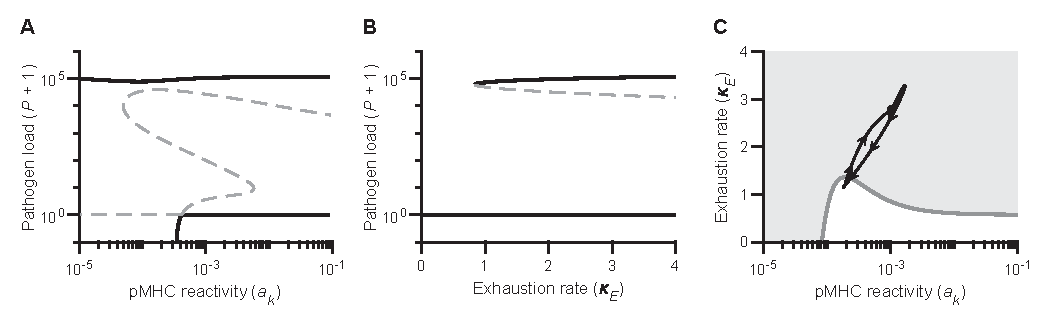
\includegraphics[width=\textwidth]{Figures/AvC/figS2_bfns.pdf}
    \caption[Bifurcation analysis of the one-clone system]{\textit{Bifurcation analysis of the one-clone system}. %
    \textbf{(A)}~Pathogen levels at steady state as a function of pMHC reactivity ($a_k=1/k$); solid black lines represent branches of attracting (stable) equilibria, while dashed lines represent branches of repelling (unstable) equilibria. The upper and lower levels of pathogen load can coexist (in the form of bistability) in the upper range of pMHC reactivity; which one of these two steady states can be attained depend on the initial conditions of pathogen load and T cell count. %
    %
    \textbf{(B)}~Pathogen levels at steady state as a function of the pathogen-dependent effector T cell depletion, $\kappa_E$, when $a_k=10^{-2.98}$; as before, solid black lines represent branches of attracting (stable) equilibria, while dashed lines represent branches of repelling (unstable) equilibria. %
    %
    \textbf{(C)}~Two-parameter bifurcation of steady state level of pathogen load with respect to the depletion rate $\kappa_E$ and pMHC reactivity parameter, $a_k$. Gray-shaded region represents the regime of coexistence between the upper and lower levels of pathogen load (i.e., the bistable regime) seen in (A) and (B). Overlaid is the trajectory of the average pMHC reactivity and average depletion rate of the ensemble of T cells of the full system, starting from the filled black circle (arrows indicate direction of motion).}
    \label{fig:AvC_supp_bfns}
\end{figure}

\begin{figure}
    \centering
    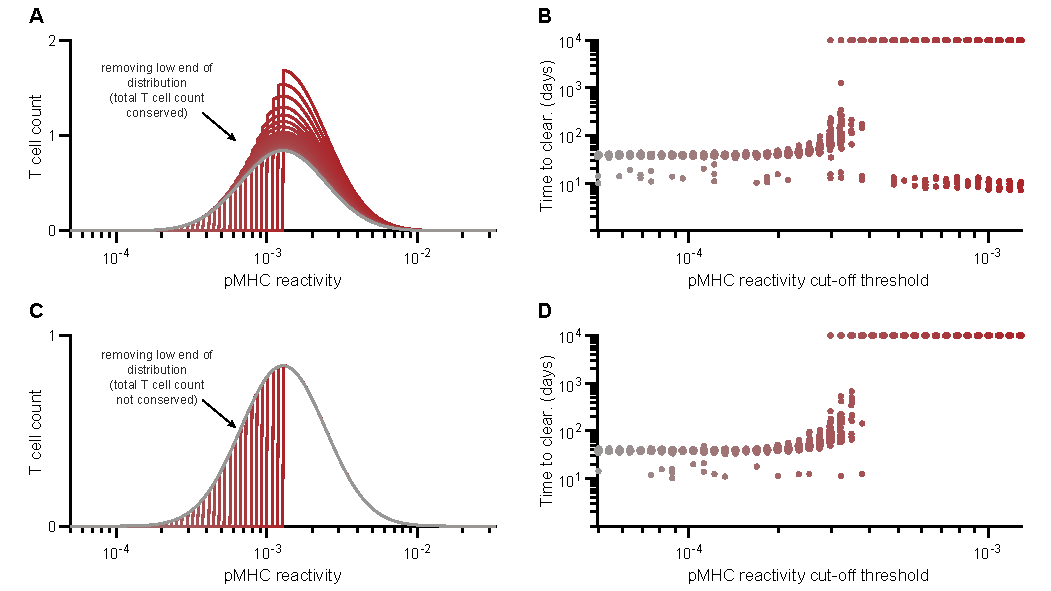
\includegraphics[width=\textwidth]{Figures/AvC/figS3_modelKO.pdf}
    \caption[Effects of removing T cells with low pMHC-reactivity]{\textit{Effects of removing T cells with low pMHC-reactivity}. %
    %
    \secbfcolor{(A)}~Distributions of initial T cell count prior to infection as a function of pMHC reactivity obtained by successively removing low-reactivity T cells using different cut-off thresholds from the model’s pre-infection repertoire and by reducing the pathogen replication rate $r_P$ to 1.16~day$^{-1}$ from its default value. Note that, since reducing $r_P$ does not affect the initial T cell count, these distributions are identical to those shown in Fig.~\ref{fig:AvC_modelKO}. %
    %
    \secbfcolor{(B)}~Time to pathogen clearance as a function of the cut-off threshold for T cell reactivity shown in (A). For each cut-off threshold, 50 simulation trials were performed as described in Fig.~\ref{fig:AvC_modelKO}. Notice the prominence of the acute cluster at high cut-off thresholds owing to a greater number of T cells with high pMHC reactivity; interestingly, this feature is not present in Fig.~\ref{fig:AvC_modelKO}B. %
    %
    \secbfcolor{(C)}~Distribution of T cell count prior to infection and with $r_P$ reduced to 1.16~day$^{-1}$, without keeping the total number of T cells conserved when removing the low-reactivity T cells at different cut-off thresholds. %
    %
    \secbfcolor{(D)}~Time to clearance as a function of the cut-off threshold of the pMHC reactivity shown in (C). Notice the disappearance of the acute cluster seen in (B) at high cut-off threshold values.}
    \label{fig:AvC_supp_modelKO}
\end{figure}

\begin{figure}
    \centering
    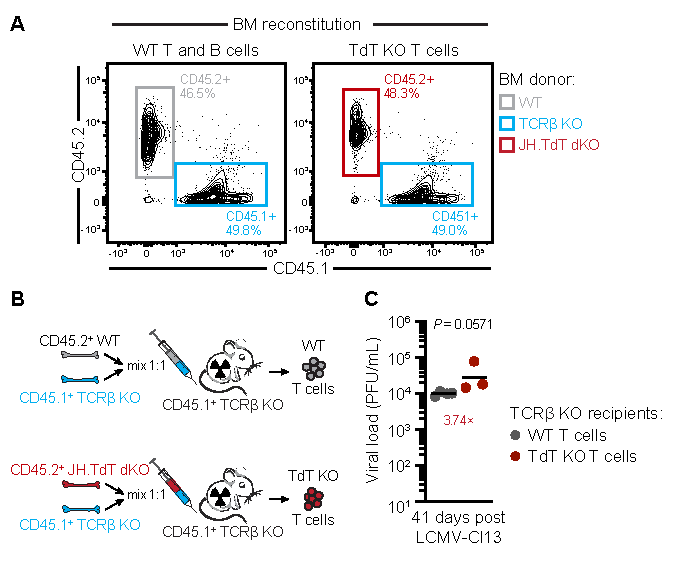
\includegraphics[width=0.64\textwidth]{Figures/AvC/figS4_tdtKO.pdf}
    \caption[Generating bone marrow chimeric mice lacking TdT in T cells only]{\textit{Generating bone marrow chimeric mice lacking TdT in T cells only}. %
    %
    \secbfcolor{(A)}~Representative flow cytometry plots showing the percent of bone marrow cells from each set of donor mice, namely CD45.1\pos{} cells from TCR\textbeta{} KO mice and CD45.2\pos{} cells from either WT or JH$\times$TdT double KO mice. %
    %
    \secbfcolor{(B)}~Modified experimental approach from Fig.~\ref{fig:AvC_tdtKO} by using TCR\textbeta{} KO mice as irradiated bone marrow recipients. %
    %
    \secbfcolor{(C)}~LCMV-Cl13 viral loads in the serum of recipient TCR\textbeta{}\KO{} mice reconstituted with WT or TdT KO T cells at day 41 post infection. P-value indicated was computed using two-tailed Wilcoxon rank sum test on geometric means.}
    \label{fig:AvC_supp_tdtKO}
\end{figure}

\begin{figure}
    \centering
    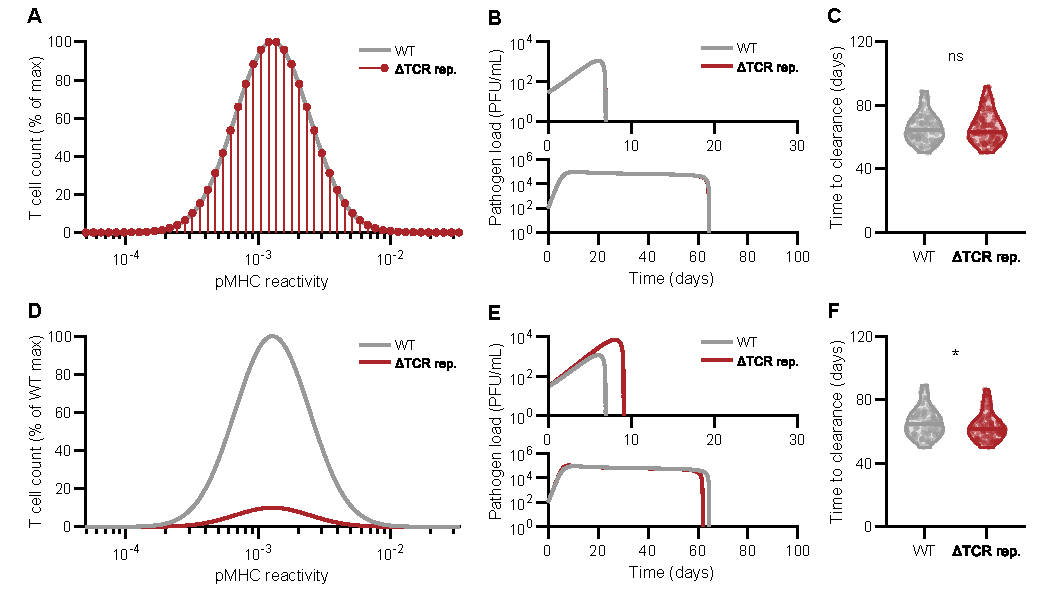
\includegraphics[width=\textwidth]{Figures/AvC/figS5_alternativeKO.pdf}
    \caption[Alternative changes to the TCR repertoire in the model produce outcomes that do not match the data in mice with TdT-deficient T cells]{\textit{Alternative changes to the TCR repertoire in the model produce outcomes that do not match the data in mice with TdT-deficient T cells}. %
    %
    \secbfcolor{(A,~D)}~Altered TCR repertoire obtained by either reducing the number of clonotypes by decreasing $N$ to 50, resulting in fewer clones across the entire pMHC reactivity range while keeping the total T cell count constant (A), or reducing precursor frequency across all pMHC reactivity values by decreasing $\sigma_{E,\textrm{tot}}$ 10-fold to 2.97 cells~day$^{-1}$ (D). %
    %
    \secbfcolor{(B,~E)}~Model simulations comparing representative pathogen load traces of WT (gray) and \dTCR{} repertoires (red) configurations in in A and C during acute (top) or chronic (bottom) infection when the number of clones is reduced (B) or when precursor frequencies are reduced (E). %
    %
    \secbfcolor{(C,~F)}~Time to clearance of chronic infections for 100 model simulations from WT and \dTCR{} repertoire systems associated with reducing number of clones (C) or precursor frequencies (F). ns, P = 0.78; *, P = 0.036. P-values computed using the Wilcoxon rank sum test.}
    \label{fig:AvC_supp_alternativeKO}
\end{figure}

\begin{figure}
    \centering
    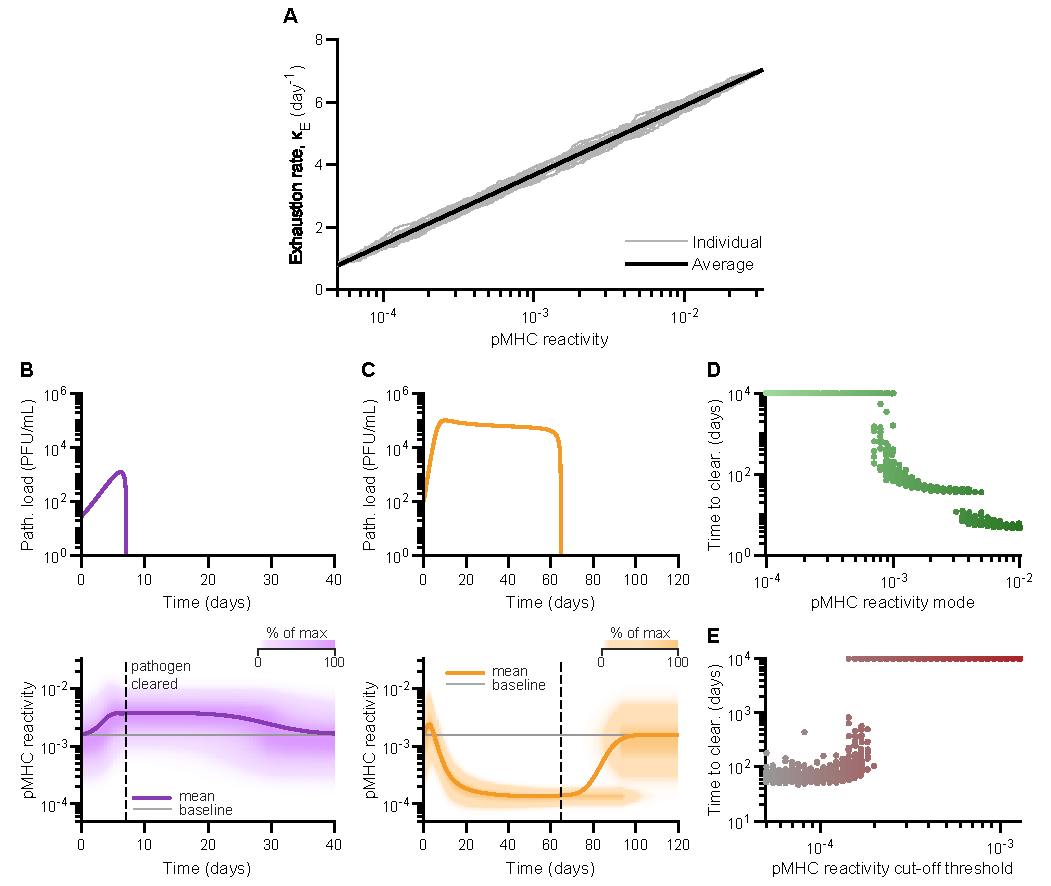
\includegraphics[width=\textwidth]{Figures/AvC/figS6_uniformExhaustion.pdf}
    \caption[Exhaustion rates sampled from a uniform distribution do not qualitatively alter model results]{\textit{Exhaustion rates sampled from a uniform distribution do not qualitatively alter model results}. %
    %
    \secbfcolor{(A)}~Function depicting pMHC reactivity-dependent exhaustion rate, $\kappa_E$, when sampling from a uniform distribution (with a lower bound of $\kappa_{E,\textrm{min}}$ as in Table~\ref{tab:AvC_parameters}, and upper bound $\kappa_{E,\textrm{max}}$ set to 6.67~day$^{-1}$) and sorting in ascending order. %
    %
    \secbfcolor{(B,~C)}~Pathogen load (top) and pMHC-reactivity distribution (bottom) obtained by simulating the model response to acute (B) or chronic (C) pathogen, when $\kappa_E$ was sampled from uniform distribution. Chronic replication rate ($r_P$) was reduced to 1.15~day$^{-1}$; all other parameters were kept at their default values shown in Table~\ref{tab:AvC_parameters}. %
    %
    \secbfcolor{(D,~E)}~Effect of varying the pMHC-reactivity mode (D), as in Fig.~\ref{fig:AvC_dists}A, or of removing T cells with low pMHC-reactivity (E), as in Fig.~\ref{fig:AvC_modelKO}B, when $\kappa_E$ was sampled from uniform distribution. Note that all results are consistent with those obtained by sampling $\kappa_E$ from an exponential distribution as shown in Fig.~\ref{fig:AvC_scheme}C.}
    \label{fig:AvC_supp_uniformExhaustion}
\end{figure}

\clearpage
\clearpage

\subsection{Model parameters and fitting}
\label{sec:AvC_modelParsFitting}

In order to generate parameter values for model simulations, a genetic algorithm was used. The fitness function of the genetic algorithm was primarily based on minimizing the sum of squared errors between the data and model predictions (i.e., minimizing $\sum_i(\mathbf{Y}_i-F(t;\mathbf{P}))^2$ , where $\mathbf{Y}_i$ is the serum time series data in~\cite{wherry2003viral}, and $F(t;\mathbf{P})$ is the fit output as a function of time with input parameter vector $\mathbf{P}$). The results were then refined to ensure the final selected parameter values satisfied the following conditions:
\begin{itemize}
    \item The pathogen replication rate for chronic LCMV (LCMV-Cl13) is larger than that for acute LCMV (LCMV-Arm), as suggested by~\cite{bergthaler2010viral,sullivan2011point}
    \item Pathogen load starts from a perturbed initial value $P_0$ (a fitted parameter, see below), and the rate of change of pathogen is initially positive i.e., $\textrm{d}P/\textrm{d}t>0$ at $t=0$.
    \item The steady state of the pathogen-free equilibrium is stable (see “Stability analysis” section below).
    \item An upper bound for the standard deviation of the function describing the $\sigma_E$ distribution, $f(k; \mu,\sigma)$, is applied to ensure that $f$ is negligibly small for non-physiologically small values of $k$ (i.e., for pMHC reactivities that are too high).
\end{itemize}

To specify the lower and upper bounds used by the parameter sampling in the genetic algorithm, ranges from similar parameters in the effector T cell dynamics (Eq.~\eqref{eq:AvC_E}) from previous mathematical models were used~\cite{khadra2009role,jaberi2015continuum,jamaleddine2020quantifying}. In order to fit serum viral loads digitized from~\cite{wherry2003viral}, we used the early time points to inform our choices for the bounds on the replication rate, $r_P$, and the initial pathogen load, $P_0$, in the context of the LCMV-Cl13 data. This was done by assuming that T cell influence is negligible early in infection, and thus pathogen expansion during this phase of the infection to be predominantly dictated by exponential growth. In other words, we assumed that pathogen load dynamics (Eq.~\eqref{eq:AvC_P}) are governed by
%
\begin{equation*}
    \dv{P}{t} \approx r_P P
\end{equation*}
%
for $P \ll P_{\textrm{max}}$, where $P_{\textrm{max}}$ is the pathogen carrying capacity. Solving this latter equation, we obtained an approximation for $P(t)$ early in the infection, given by 
%
\begin{equation*}
    P(t) \approx P_0 \exp(r_P t) \quad \Rightarrow \quad \ln{P(t)} \approx r_P t + \ln{P_0}
\end{equation*}
%
where $P_0=P(t=0)$. Fitting this linear expression of $\ln{P(t)}$ in terms of $t$ to the digitized data in~\cite{wherry2003viral}, we obtained an estimate for the confidence bounds on $r_P$ and $\ln{P_0}$. The range used for the pathogen carrying capacity, $P_{\textrm{max}}$, was set to be on the order of $10^5$~PFU/mL, a value that is consistent with the range of values of LCMV-Cl13 titres in the serum at peak infection in the data.

The pMHC-reactivity distribution mode and span, parameters that are not identifiable but important for the study, were sampled from wide ranges by the genetic algorithm. In the case of the mode, it was sampled uniformly on a log scale, unlike the other parameters that are sampled uniformly on a linear scale. To define the distribution of thymic input defined by the log-normal function of pMHC reactivity, we let $\sigma_E(k)=\sigma_{E,\textrm{tot}} \, f(k;\mu,\sigma)$, where $f$ is the log-normal probability density function with mean and standard deviation $\mu$ and $\sigma$, respectively, and $\sigma_{E,\textrm{tot}}$ is the total thymic input of pathogen-specific T cells across all pMHC-reactivity values. The mode of the $a_k$ distributions used in Fig.~\ref{fig:AvC_dists}A is given by $1/\exp(\mu+\sigma^2)$, where $a_k=1/k$, and the span of these distributions used in Fig.~\ref{fig:AvC_dists}B is $\exp(\sigma)$.

Let $k_{\textrm{mode}}=\exp(\mu+\sigma^2)$ and $k_{\textrm{span}}=\exp(\sigma)$ be the mode and span, respectively, that define the log-normal probability density function $f$. Since these quantities are simpler to think about than $\mu$ and $\sigma$ themselves, we defined an equivalent function $\sigma_E(k)=\sigma_{E,\textrm{tot}} \, \Tilde{f} (k;k_{\textrm{mode}},k_{\textrm{span}})$. The parameters $k_{\textrm{mode}}$ and $k_{\textrm{span}}$ are the parameters that were fit by the genetic algorithm. We assigned the upper and lower bounds on $k$ ($k_{\textrm{max}}$ and $k_{\textrm{min}}$, respectively) to be at $\pm 5\sigma$ in log space from the fitted mode $k_{\textrm{mode}}$.


\subsection{Numerical simulation}
\label{sec:AvC_numericalSimmulation}

To simulate the system of integro-differential equations, we discretized the continuous T cell population $E(t,k)$, into individual clones of T cells $E_i$ with pMHC reactivity $a_{k,i} = 1/k_i$, where $i=1,2,...,N$ and $N$ is the number of T cell clonotypes. To approximate a pMHC-reactivity continuum, we chose a large value for $N$. The resulting model becomes a high-dimensional system of ordinary differential equations with $N+1$ variables, whose equations can be expressed as
%
\begin{align*}
    \dv{P}{t} &= r_P P \left(1 - \frac{P}{P_{\textrm{max}}}\right) - \kappa_P \sum_{i=1}^N E_i \frac{P}{P+a \, k_i}, \\[0.5em]
    \dv{E_i}{t} &= \sigma_E(k_i) + r_E E_i \frac{P}{P+k_i} - \delta_E E_i - \kappa_E(k_i) E_i \frac{P}{P+b \, k_i} - \varepsilon E_i \sum_{j=1}^N E_j.
\end{align*}
%
To initialize the simulations, we first allowed $E_i$ to evolve toward their baseline values in the absence of pathogen, i.e., when $P=0$ as described in the next section. Then, we introduced a non-zero perturbation to the pathogen load at time $t=0$, i.e., $P(t=0)\rightarrow P_0$ where $P_0$ is obtained from parameter fitting as described previously.


\subsection{Stability analysis of the full model}

One can show that $(P,\boldsymbol{E})=(0,\boldsymbol{E^*})$, where $\boldsymbol{E^*}=(E_1^*,E_2^*,...,E_N^*)$ is the level of each effector T cell clone in the pathogen-free equilibrium, is always a steady state solution of the full, discretized system. We denoted this steady state by $\boldsymbol{S_0}$, which represents the state of the system at homeostasis, i.e., in the absence of pathogen. Since we did not explicitly incorporate a memory formalism into the mathematical model, $\boldsymbol{S_0}$ is both the baseline state that effector T cells are initialized from prior to the introduction of pathogen, as well as the state that the system evolves to upon pathogen clearance. Note that $\boldsymbol{S_0}$ is distinct from the initial state of the model upon infection, which begins at $(P,\boldsymbol{E})=(P_0,\boldsymbol{E^*})$, as described above. In this section, we will determine the condition needed to ensure that $\boldsymbol{S_0}$ is stable. This condition is then imposed on the genetic algorithm when evaluating parameter fitness.

The Jacobian matrix of the full system evaluated at the steady state $\boldsymbol{S_0} = (0, \boldsymbol{E^*})$ can be written as
%
\setlength{\arraycolsep}{1.6mm}
\begin{equation*}
    \mathbf{J}_{\boldsymbol{S_0}} = 
    \begin{pmatrix}
        r_P - \dfrac{\kappa_P}{a} \displaystyle\sum_{n=1}^N \dfrac{E_n^*}{k_n} & 0 & 0 & ... & 0 \\[1.5em]
        %
        \dfrac{E_1^*}{k_1}\left( r_E - \dfrac{\kappa_E}{b} \right) & -\delta_E - \varepsilon E_1^* - \varepsilon \displaystyle\sum_{n=1}^N E_n^* & - \varepsilon E_1^* & ... & - \varepsilon E_1^* \\[1.5em]
        %
        \dfrac{E_2^*}{k_2}\left( r_E - \dfrac{\kappa_E}{b} \right) & - \varepsilon E_2^*  & -\delta_E - \varepsilon E_2^* - \varepsilon \displaystyle\sum_{n=1}^N E_n^* & ... & - \varepsilon E_2^* \\[1.5em]
        %
        \vdots & \vdots & \vdots & \ddots & \vdots \\[1.5em]
        %
        \dfrac{E_N^*}{k_N}\left( r_E - \dfrac{\kappa_E}{b} \right) & - \varepsilon E_N^* & - \varepsilon E_N^* & ... & -\delta_E - \varepsilon E_N^* - \varepsilon \displaystyle\sum_{n=1}^N E_n^*
    \end{pmatrix}.
\end{equation*}
%
The eigenvalues of this Jacobian matrix are given by
%
\begin{align*}
    \lambda_0 &= r_P - \frac{\kappa_P}{a} \sum_{n=1}^N \frac{E_n^*}{k_n},\\[0.5em]
    \lambda_1 &= -\delta_E - 2\varepsilon\sum_{n=1}^N E_n^*, \quad \textrm{and}\\[0.5em]
    \lambda_i &= -\delta_E - \varepsilon\sum_{n=1}^N E_n^* \quad \textrm{for} \quad i\in\{2,3,...,N\}.
\end{align*}
%
It follows that $\lambda_0<0$ is a necessary and sufficient condition to ensure local stability of $\boldsymbol{S_0}$, as all other eigenvalues are always negative for positive parameter values and T cell levels. This condition may be rewritten as
%
\begin{equation*}
    \sum_{n=1}^N \frac{E_n^*}{k_n} > \frac{r_P \, a}{\kappa_P}.
\end{equation*}
%
The individual values of $E_n^*$ may be computed by simulating the full model in the absence of pathogen (i.e., for $P=0$); this condition can then be verified during the parameter fitness evaluation process of the genetic algorithm to reject parameter selections that do not ensure the stability of $\boldsymbol{S_0}$.

The existence and stability of other steady states in the model depends on different parameter values. To assess them, we employed a bifurcation analysis approach applied on a simplified single-clone ($N=1$), 2-dimensional model.


\subsection{Analysis of the reduced one-clone, 2D model}
\label{sec:AvC_2DmodelAnalysis}

To better understand the underlying dynamics of the full continuum model and the distinct time scales between outcomes of an acute and chronic infection, we turned our attention to a simplified, single-clone version of the model (with $N=1$), given by
%
\begin{align*}
    \dv{P}{t} &= r_P P \left(1 - \frac{P}{P_{\textrm{max}}}\right) - \kappa_P \sum_{i=1}^N E_i \frac{P}{P+a \, k}\,\,, \\[0.5em]
    \dv{E}{t} &= \sigma_E+ r_E E \frac{P}{P+k} - \delta_E E - \kappa_E E \frac{P}{P+b \, k} - \varepsilon E^2.
\end{align*}
%
Model parameters were assigned the same values as those provided in Table~\ref{tab:AvC_parameters}, except for $\sigma_E$, $\kappa_E$ and $k$. In this case, $\sigma_E$ was set to be 29.7~cells/day, $\kappa_E$ to be 2.78~day$^{-1}$ and $k$ to be a bifurcation parameter spanning a wide range.

Figure~\ref{fig:AvC_supp_bfns}A plots the steady-state levels of the pathogen load, $P$, on a log-scale, as a function of the pMHC reactivity ($a_k$). The pathogen load was shifted by 1, to show the behaviour at $P=0$ on a log-scale (i.e., $10^0$ corresponds to $P=0$). The figure shows that pathogen load can attain two different values at steady state (solid lines): an elevated level (hereafter referred to as the $\boldsymbol{S_1}$ state) and a low level ($\boldsymbol{S_0}$), both acting as attractors (as opposed to repellers shown as dashed lines) that can co-exist at high $a_k$. This coexistence of the two attractors is a hallmark of bistability, which highlights the dependence of the system on the initial level of $P$ to determine which attractor will be eventually approached over time. For the $\boldsymbol{S_0}$ steady state to be an attractor (stable), the condition $a_k > 4.15 \times 10^{-4}$ must be satisfied.\footnote{Note that units are omitted from the discussion of the pMHC-reactivity measure, since $a_k$ does not represent a direct value for the affinity of the T cell receptor but rather acts as an indicator for it.}

We next showed the behaviour of the system with respect to the pathogen-dependent effector T-cell exhaustion rate, $\kappa_E$ (Fig.~\ref{fig:AvC_supp_bfns}B). Pathogen loads can be either elevated or zero due to the presence of bistability for $\kappa_E > 0.84$~day$^{-1}$. Below this critical value of $\kappa_E$, only the lower steady state exists as the system’s global attractor.\footnote{Within the physiological range of the system, $P \ge 0$ and $E \ge 0$.}

To understand the effects of such dynamics of the single-clone model on the full, continuum model, we computed the evolution of the weighted average of pMHC reactivity and that of the exhaustion rate of dominant effector T cells throughout the chronic immune response and overlaid this trajectory on the 2-parameter bifurcation diagram of viral load with respect to $\kappa_E$ and $a_k$ of the single clone model (Fig.~\ref{fig:AvC_supp_bfns}C). The gray-shaded region represents the bistable region in Fig.~\ref{fig:AvC_supp_bfns}B. The starting values of the average exhaustion rates and pMHC reactivities fall within the bistable region; acute vs. chronic outcomes are set apart by whether the system evolves immediately toward $\boldsymbol{S_0}$ (acute), or if it first goes to the upper $\boldsymbol{S_1}$ state and can only come back down once the full system moves out of the gray region. The latter, as a result, takes much longer, causing the full model to produce the time scale separation (clustering) in the time to clearance between acute vs. chronic infections.

This time scale separation observed in the full model can be further visualized by examining how the nullclines of the one-clone system dictate the dynamics of the full model when the average values of $a_k$ and  $\kappa_E$ parameters change; this was done by superimposing a solution trajectory of the full model on the phase space of the one-clone system and observing how they all evolve over time (Mov.~\ref{mov:AvC_nullclines}). Doing so revealed that, during a chronic infection, the trajectory evolves toward a transiently existing stable steady state with elevated pathogen load (i.e., toward $\boldsymbol{S_1}$). The fixed point $\boldsymbol{S_1}$, however, eventually disappears at a saddle-node bifurcation as the average pMHC reactivity and exhaustion rate parameters of the full model decrease, leading the solution trajectory to return back to $\boldsymbol{S_0}$ (where the $E$-nullcline meets the vertical $P$-nullcline). Note that the initial state of the simulations from which the numerical solution is computed, i.e., the small perturbation $P_0$ located horizontally to the right of $\boldsymbol{S_0}$, falls under the parabolic $P$-nullcline, allowing the pathogen to grow initially. Whether the solution follows a small loop before returning to $\boldsymbol{S_0}$ (acute), or evolves toward the transiently existing $\boldsymbol{S_1}$ (chronic), depends on whether the initial condition lies to the left or to the right, respectively, of the saddle fixed point’s stable manifold.

Of note, the equations representing effector T cell dynamics, and the resulting bifurcation diagram, bear resemblance to the model studying post-treatment control of HIV-1 infection described in~\cite{conway2015post}. In that study, bistability was also an important feature of the model, explaining how some individuals infected with HIV-1 could maintain undetectable viral loads after cessation of anti-retroviral treatment. However, our model differs in that we do not observe a third stable state with non-zero albeit undetectable low pathogen loads.

\renewcommand{\thetable}{\thechapter.\arabic{table}}
\setcounter{table}{0}

\renewcommand{\thefigure}{\thechapter.\arabic{figure}}
\renewcommand{\figurename}{Figure}
\setcounter{figure}{0}